\chapter[Continuação analítica]{Continuação analítica}
\chaptermark{}

\hfill%
\begin{minipage}{10cm}
    \begin{flushright}
    \rightskip=0.5cm
        \textit{``The greatest strategy is doomed if it's implemented badly.''}
        \\[0.1cm]
    \rightskip=0.5cm
    --- Bernhard Riemann
    \end{flushright}
\end{minipage}

\section{O logaritmo de uma função}

    Vamos investigar se é possível definir o logaritmo complexo para uma função holomorfa 
    $f: G \to \C$, onde $G$ é um domínio contendo a origem. Caso tal construção fosse possível,
    então $\log f(z)$ seria a primitiva de $f'(z)/f(z)$. O princípio do argumento nos mostra que
    %
    \begin{equation*}
        \int_\y \frac{f'(z)}{f(z)} dz = 2\pi i K,
    \end{equation*}
    %
    onde $\y$ é uma curva fechada e $K$ é um inteiro. Isto significa que $\log f(z)$ muda 
    de um tanto $2\pi i K$ cada vez que a variável $z$ percorre $\y$; como consequência disso,
    a parte imaginária do logaritmo (o argumento) muda de um tanto $2 \pi K$. No entanto, uma
    função holomorfa que admite uma primitiva é tal que sua integral ao longo de uma curva fechada
    é sempre nula. Isto mostra que deveríamos ter
    %
    \begin{equation*}
        \int_\y \frac{f'(z)}{f(z)} \, dz = 0,
    \end{equation*}
    o que nos mostra que não podemos definir $\log f(z)$.
    
    De uma forma mais precisa, definir o logaritmo para a função $f$ significa escolher um ramo 
    do logaritmo em $G$, i.e., uma função $g: G \to \C$ tal que 
    %
    \begin{equation*}
        \exp(g(z)) = f(z), \forall z \in G.  
    \end{equation*}
    %
    Já vimos que esta construção não será possível por conta do princípio do argumento, mas a
    seguir faremos uma tentativa de definir tal função e veremos em detalhes por que não é 
    possível fazê-la.
    
    Vamos tratar de um caso específico em que $G$ é um domínio contendo a origem e 
    $\y: [0,1] \to \C$ é uma circunferência com centro em $0$, $\y = r\exp{2 \pi i t}$, 
    em que $r > 0$ é tal que os pontos de $\y$ estão em $G$. Vamos supor que $f$ tem apenas 
    uma singularidade $z_0$ no interior da região delimitada por $\y$. Sendo $\y$ uma
    aplicação contínua, temos que a curva que ela parametriza é um compacto de $\C$, pois é o
    conjunto $\y([0,1])$ e $[0,1]$ é compacto em $\R$. Isso significa que podemos escolher um
    número finito de bolas $B_i$ centradas nos pontos $\y(t_i)$, com $t_i \in [0,1]$ e 
    $i \in \{1,\dots, n\}$. Vamos supor que $t_1 < t_2 < \cdots < t_n$ e que 
    $\y(t_1) = \y(t_n)$.  Os raios das bolas $B_i$ podem ser escolhidos todos iguais a
    algum $\e > 0$ tal que $z_0 \not \in B_i$ e $B_i \subseteq G$ para todo $i$.
    
    A ideia é escolher, para cada $i$, um ramo $\mathcal{L}_i$ do logaritmo em $\C$ tal que 
    $\log f(z)$ esteja bem definido na bola $B_i$. Essa escolha deve ser feita de tal modo que
    $\mathcal{L}_i$ e $\mathcal{L}_{i+1}$ coincidam na interseção $B_i \cap B_{i+1}$ para todo $i$.
    Dessa forma, usando o princípio da identidade, vamos definir $\log f(z)$ estendendo o primeiro
    ramo analiticamente para os outros ramos em um subconjunto de $G$ que não contém $z_0$. 
    É importante excluir $z_0$, pois $\log$ não está definido em $0$ em nenhum ramo.
    
    Denote $a_i = \y(t_i)$. Vamos mostrar que podemos definir $\log f(z)$ em $B_i$. 
    O que precisamos aqui é que seja possível escolher uma semirreta 
    $L_\phi = \{s(\cos \phi, \sen \phi): s > 0\}$ que não intercepte $f(B_i)$; caso contrário, 
    não poderíamos definir a imagem de todos os pontos de $f(B_i)$ por um mesmo ramo do logaritmo.
    Nesta parte a discussão fica um pouco mais técnica, então vamos apenas enunciar o resultado 
    que usaremos. 
    %
    \begin{teorema}
        Seja $f: G \to \C$ uma função holomorfa, onde $G$ é um domínio. 
        Se $U \subseteq G$ é um aberto tal que $\overline{U} \subseteq G$, então
        \begin{itemize}
            \item $f(\partial U) \subseteq \partial f(U)$;
            \item $f(U)$ é aberto.
        \end{itemize}
    \end{teorema}
    %
    Faremos a hipótese adicional daqui em diante de que $\overline{B}_i \subseteq G$. 
    Este teorema nos permite concluir que podemos, de fato, escolher algum $L_\phi$ 
    bom o bastante para definir o ramo $\mathcal{L}_i$. Observe ainda que $0 \not \in f(B_i)$.
    
    Passemos agora à construção de $\log f(z)$. Começamos com $B_1$ centrado em $\y(t_1)$
    escolhendo um ramo $\mathcal{L}_1$ adequado, denotamos a semirreta $L_\phi$ correspondente por
    $L_{\phi_1}$. Para o próximo ramo, $\mathcal{L}_2$, escolhemos $\phi_2$ tal que $L_{\phi_2}$
    não intercepte a interseção $f(B_1) \cap f(B_2)$. Dessa forma, 
    $\log_{\phi_1} f(z) = \log_{\phi_2} f(z)$ para todo $z$ nesta interseção. 
    Neste ponto, conseguimos definir $\log f(z)$ em $B_1 \cup B_2$ da seguinte forma:
    %
    \begin{equation*}
        \log f(z) =
        \begin{cases}
            \log_{\phi_1} f(z), z \in B_1 \\
            \log_{\phi_2} f(z), z \in B_2.
        \end{cases}
    \end{equation*}
    %
    Continuamos dessa maneira e fazemos agora o mesmo para a escolha de $L_{\phi_3}$, 
    restringindo nossa atenção à interseção $f(B_2) \cap f(B_3)$. Por simplicidade, 
    vamos escrever $l_i(z) =  \log_{\phi_i} f(z)$. Observe que, como $a_n = a_1$, 
    definiremos um total de $n-1$ ramos do logaritmo. Quando chegarmos na última bola, 
    $B_n \ (= B_1)$, temos uma condição de compatibilidade adicional a ser verificada. 
    Devemos ter $l_{n-1}(z) = l_1(z)$ para todo $z$ em $B_{n-1} \cap B_1$. Vamos supor que isso
    tenha sido feito com sucesso.
    
    Denote por $\y_j$ a função $\y$ restita ao intervalo $[t_{j-1},t_j]$, ou seja, ela
    parametriza o pedaço de $\y$ que vai de $a_{j-1}$ para $a_j$. Adicionamos daqui em diante 
    a hipótese de que $a_i$ e $a_{i+1}$ são pontos de $B_i$ para todo $i$. Pelo teorema fundamental
    do cálculo, temos
    %
    \begin{equation*}
        \int_{\y_j} = \frac{f'(z)}{f(z)}\, dz = l_j(a_j) - l_j(a_{j-1}).  
    \end{equation*}
    %
    Integrando em $\y$ e usando o princípio do argumento, obtemos
    \begin{align*}
        2 \pi i K &= \int_{\y} = \frac{f'(z)}{f(z)}\, dz \\
        &= \sum_{j=1}^{n-1}\int_{\y_j} = \frac{f'(z)}{f(z)}\, dz \\
        &= [l_1(a_2) - l_1(a_1)] + [l_2(a_3) - l_2(a_2)] + \cdots \\
        &+ [l_{n-2}(a_{n-1}) - l_{n-2}(a_{n-2})] + [l_{n-1}(a_{n}) - l_{n-1}(a_{n-1})] \\
        &= l_{n-1}(a_n) - l_1(a_1)\\
        &= 0,
    \end{align*}
    onde $K$ é a multiplicidade do zero $z_0$ de $f$. Observe que as condições de compatibilidade,
    que são satisfeitas por construção ($l_i$ e $l_{i+1}$ são coincidentes na interseção 
    $B_i \cap B_{i+1}$), fazem com que a soma acima tenha vários cancelamentos, restando apenas o
    termo na penúltima igualdade. A soma então se anula por conta da condição de compatibilidade
    adicional que supomos ser satisfeita ($l_{n-1}(z) = l_1(z)$ para todo $z$ em 
    $B_{n-1} \cap B_1$). Lembre-se ainda que $a_1 = a_n$.
    
    Por esta contradição, concluímos que não podemos definir $\log f(z)$ desta forma que fizemos.
    Este é apenas um caso particular, mas mostra um pouco do por quê não é possível fazer tal
    construção.

\section{Continuação analítica ao longo de caminhos}

% fazer a discussão introdutória (slides da Aula 1 e início dos slides da Aula 2)

    \begin{definicao}
        \label{def-elemento-funcao}
        Um elemento de função é um par $(f, G)$ onde $G$ é um domínio e $f$
        é uma função analítica em $G$. Dado um elemento de função $(f,G)$, 
        definimos o germe de $f$ em $a$, denotado por $[f]_a$, 
        como a coleção de todos os elementos de função $(g,D)$ tais que 
        $a\in D$ e $f(z) = g(z)$ para todo $z$ em uma vizinhança de $a$.
    \end{definicao}


    \begin{definicao}
    \label{def-continuacao-analitica}
        Seja $\y: [0,1] \to \C$ um caminho e suponha que para cada
        $t\in[0,1]$ existe um elemento de função $(f_t, D_t)$ tal que
        \begin{enumerate}[(a)]
            \item $\y(t) \in D_t$;
            \item para cada $t\in[0,1]$ existe $\delta > 0$ tal que se $|s-t| < \delta$
            então $\y(s) \in D_t$ e $[f_s]_{\y(s)} = [f_t]_{\y(s)}$.
        \end{enumerate}
        Nesse caso, dizemos que $(f_1, D_1)$ é a continuação analítica de $(f_0,D_0)$ ao 
        longo de $\y$ ou ainda que $(f_1, D_1)$ é obtido a partir de $(f_0,D_0)$ por
        continuação analítica ao longo de $\y$.
    \end{definicao}


    \begin{proposicao}
    \label{prop-unicidade-continuacao-analitica-caminho}
        Seja $\y: [0,1]\to\C$ um caminho de $a$ para $b$ e sejam
        \begin{align*}
            \left\{ (f_t, D_t): 0\leq t\leq 1 \right\}, \\
            \left\{ (g_t, B_t): 0\leq t\leq 1 \right\}
        \end{align*}
        continuações analíticas ao longo de $\y$ tais que $[f_0]_a = [g_0]_a$.
        Então $[f_1]_b = [g_1]_b$.
    \end{proposicao}

    \begin{proof}
        A ideia é mostrar que
        %
        \begin{equation*}
            T = \left\{ t\in [0,1] : [f_t]_{\y(t)}= [g_t]_{\y(t)} \right\}
        \end{equation*}
        %
        é aberto e fechado em $[0,1]$ (com a topologia induzida pela topologia usual da reta).
        Isso, juntamente aos fatos de que $T$ é não-vazio ($0\in T$) e $[0,1]$ é conexo, 
        nos permitirá concluir que $T = [0,1]$ e, em particular, $1\in T$.
        
        Para mostrar que $T$ é aberto, seja $t\in T$ não nulo e diferente de 1 
        (se $t=1$ terminamos). Por definição de continuação analítica, existe $\delta > 0$
        tal que se $|s-t|<\delta$ então $\y(s) \in D_t\cap B_t$ e
        %
        \begin{equation*}
            \begin{cases}
            [f_s]_{\y(s)} = [f_t]_{\y(s)} \\
            [g_s]_{\y(s)} = [g_t]_{\y(s)}.
            \end{cases}
        \end{equation*}
        %
        Seja $H\subseteq D_t\cap B_t$ tal que $\y(s), \y(t)\in H$. 
        %
        \begin{center}
            \textbf{diagrama slide 17 aula 2}
        \end{center}
        %
        Como $t\in T$,
        $f_t(z) = g_t(z), \forall z\in H$. Logo, $[f_t]_{\y(s)} = [g_t]_{\y(s)}$
        para todo $\y(s)\in D_t\cap D_s$. Segue então das duas igualdades acima que
        $[f_s]_{\y(s)} = [g_s]_{\y(s)}$ se $|s-t|<\delta$. Logo, 
        $(t-\delta, t+\delta)\subseteq T$ e, como $t$ é um ponto qualquer de $T$, temos
        $T$ aberto em $[0,1]$.
        
        Agora, para mostrar que $T$ é também fechado em $[0,1]$, tome $t$ um ponto 
        limite de $T$ e escolha $\delta>0$ tal que $\y(s) \in D_t\cap B_t$ e
        %
        \begin{equation*}
            \begin{cases}
                [f_s]_{\y(s)} = [f_t]_{\y(s)} \\
                [g_s]_{\y(s)} = [g_t]_{\y(s)}.
            \end{cases}
        \end{equation*}
        %
        sempre que $|s-t|<\delta$. Como $t$ é ponto limite de $T$, existe $s\in T$ com
        $|s-t|<\delta$. Seja então $G$ um domínio tal que 
        $\y((t-\delta, t+\delta))\subseteq G\subseteq D_t\cap B_t$.
        Em particular, temos $\y(s)\in G$ e, por definição de $T$, segue que
        $f_s(z) = g_s(z), \forall z\in G$. Usando novamente as duas igualdades anteriores, 
        podemos garantir que
        %
        \begin{equation*}
            \begin{cases}
                f_s(z) = f_t(z) \\
                g_s(z) = g_t(z)
            \end{cases}, \forall z\in G
        \end{equation*}
        %
        donde segue que $f_t(z) = g_t(z), \forall z\in G$. Ora, já que $G$ é aberto 
        (e portanto possui um ponto limite em $D_t\cap B_t$), segue que 
        $[f_t]_{\y(t)} = [g_t]_{\y(t)}$, ou seja, $t\in T$ e, consequentemente,
        $T$ contém todos os seus pontos limites, i.e., é fechado.
    \end{proof}


    \begin{observacao}
        Note que o caminho $\y$ na 
        Proposição \ref{prop-unicidade-continuacao-analitica-caminho} é o
        mesmo para $f$ e $g$! Isso será muito relevante a seguir devido ao 
        seguinte exemplo.
        
        Defina $\arg_0: \left\{ z\in\C : \Re(z) > 0 \right\} \to (-\pi/2, \pi/2)$,
        que é uma restrição do ramo principal do argumento a um domínio mais ``restrito''.
        %
        \begin{center}
            \textbf{diagrama slide 4 aula 3}
        \end{center}
        %
        Considere também a função analítica 
        $f: \left\{ z\in\C : \Re(z) > 0 \right\} \to\C$
        dada por $f(z) = \ln(z) + i\arg_0(z)$.
        %
        \begin{center}
            \textbf{diagrama slide 5 aula 3}
        \end{center}
        %
        Vamos definir na região do diagrama da esquerda uma continuação analítica
        \begin{equation*}
            \left\{ (f_t, D_t), t\in [0,1] \right\}
        \end{equation*}
        ao longo de $\y_1$, com $-1\in D_1$, $f_1(-1) = i\pi/2$,
        $D_0 = \left\{ z\in\C : \Re(z) > 0 \right\}$ e $f_0 = f$.
        
        Na região mostrada no diagrama da direita, vamos definir uma continuação analítica
        $\left\{ (g_t, B_t), t\in [0,1] \right\}$ ao longo de $\y_2$,
        com $-1\in B_1$, $g_1(-1) = -i\pi/2$, 
        $B_0 = \left\{ z\in\C : \Re(z) > 0 \right\}$ e $g_0 = f$.
        
        Note que podemos usar essas continuações analíticas para construir duas
        \textbf{extensões analíticas} $F:U_1\to\C$ e $G:U_2\to\C$, 
        com $F(z) = f_t(z), z\in D_t$ e $G(z) = g_t(z), z\in B_t$, 
        sendo $U_1$ e $U_2$ as uniões do domínio original de $f$
        com as regiões azul e vermelha, respectivamente. Ora, mas note que
        $F$ e $G$, apesar de coincidirem no domínio original de $f$, são distintas!
        
        Esse fato parece, à primeira vista, contradizer o princípio da identidade. 
        Entretanto, isso não acontece porque $F$ e $G$ não estão definidas no mesmo
        domínio. À segunda vista, pode parecer que a conclusão em que chegamos contradiz
        a Proposição \ref{prop-unicidade-continuacao-analitica-caminho}. Mas isso também 
        não ocorre, porque $F$ e $G$ foram construídas por caminhos distintos!
    \end{observacao}


    \begin{definicao}
    \label{def-continuacao-analitica-germe}
        Se $\y: [0,1]\to\C$ é um caminho de $a$ para $b$ e 
        $\left\{ (f_t, D_t): 0\leq t\leq 1 \right\}$ é uma continuação analítica ao
        longo de $\y$, então o germe $[f_1]_b$ é a continuação analítica de
        $[f_0]_a$ ao longo de $\y$.
    \end{definicao}

    Note que é preciso usar a Proposição \ref{prop-unicidade-continuacao-analitica-caminho}
    para verificar que a definição acima está bem posta. Ademais, note que ela torna
    as coisas mais práticas, pois nos permite simplificar a descrição dos $D_t$'s.

    \begin{observacao}
        Sejam $U_1, U_2\subseteq\C$ domínios não-vazios tais que $U_1\cap U_2$
        também é um domínio não-vazio.
        %
        \begin{center}
            \textbf{diagrama slide 9 aula 3}
        \end{center}
        %
        Sejam ainda $f:U_1\to\C$ e $g:U_2\to\C$ funções analíticas
        tais que $f(z) = g(z), \forall z\in U_1\cap U_2$. Nesse caso, dizemos que
        $g$ é uma continuação analítica de $f$ a $U_2$ e vice-versa: $f$ é 
        uma continuação analítica de $g$ a $U_1$.
        
        Essas duas aplicações podem ser usadas para construir uma extensão analítica
        $F: U_1\cup U_2\to\C$ dada por partes:
        %
        \begin{equation*}
            F(z) = 
            \begin{cases}
                f(z), z\in U_1; \\
                g(z), z\in U_2.
            \end{cases}
        \end{equation*}
        %
        Nesse caso, $(f,U_1)$ e $(g,U_2)$ são os elementos de função de $F$. 
        Essa é a motivação para a definição de \textit{elemento de função}.
        
        Vale reiterar que extensões analíticas por continuações analíticas distintas
        não precisam coincidir. No diagrama abaixo temos $F: U\cup V\to\C$
        e $G:U\cup W\to\C$ analíticas, com
        %
        \begin{align*}
            F(z) &= 
            \begin{cases}
                f(z), z\in U; \\
                g(z), z\in V.
            \end{cases}, \\
            G(z) &= 
            \begin{cases}
                f(z), z\in U; \\
                h(z), z\in W.
            \end{cases}
        \end{align*}
        %
        mas $F\neq G$.
        %
        \begin{center}
            \textbf{diagrama slide 11 aula 3}
        \end{center}
        %
    \end{observacao}

    Damos sequência com duas definições que, à primeira vista, não parecem ter 
    nada a ver com os termos por elas definidos.

    \begin{definicao}
    \label{def-funcao-analitica-completa}
        Se $(f,G)$ é um elemento de função, então a função analítica completa obtida
        a partir de $(f,G)$ é a coleção $\mathfrak{F}$ de todos os germes $[g]_b$ 
        para os quais existem $a\in G$ e um caminho $\y$ de $a$ para $b$ 
        tais que $[g]_b$ é a continuação analítica de $[f]_a$ ao longo de $\y$.
    \end{definicao}


    \begin{definicao}
        Uma coleção de germes $\mathfrak{F}$ é chamada função analítica completa se
        existe um elemento de função $(f,G)$ tal que $\mathfrak{F}$ é a função analítica
        completa obtida de $(f,G)$.
    \end{definicao}

    Note que esta definição nos permite ``esquecer'' do ponto $a$ mencionado na
    Definição \ref{def-funcao-analitica-completa}. Podemos escolher qualquer ponto
    de $G$, já que ele é um domínio.

    A pergunta natural a se fazer é: ``por que a terminologia de 
    \textbf{função analítica completa} é adequada quando nos referimos a uma
    coleção de germes?'', e a resposta é surpreendente. Vamos mostrar que
    podemos construir uma função a partir da coleção $\mathfrak{F}$ de germes.

    Inicialmente, consideremos a coleção
    %
    \begin{equation*}
        \mathcal{R} = \left\{ (z, [g]_z) : [g]_z \in \mathfrak{F} \right\}.
    \end{equation*}
    %
    Definimos então $\widetilde{\mathfrak{F}}:\mathcal{R}\to\C$ por
    %
    \begin{equation*}
        \widetilde{\mathfrak{F}}((z, [g]_z)) = g(z),
    \end{equation*}
    %
    ou seja, escolhemos um ``representante'' do germe e calculamos sua imagem em $z$.
    
    {\red Falar do teorema de uniformização...}

\section{Teorema de Monodromia}

    Monodromia é o estudo de como objetos da Análise, Topologia Algébrica, Geometria
    Algébrica e Geometria Diferencial se comportam à medida que 
    ``circundam uma singularidade''. O dá origem ao fenômeno de monodromia são certas
    funções que gostaríamos de definir falham em ter um valor único quando ``circulam''
    uma singularidade (e.g., o logaritmo).
    
    Como vimos acima com o exemplo do logaritmo, continuações analíticas em 
    caminhos distintos não precisam coincidir. O leitor familiar com teoria de
    homotopia poderia pensar que uma condição suficiente para a
    igualdade das continuações pode ser dada em termos dessa teoria. Entretanto,
    como todas as curvas no plano (complexo) são homotópicas, o resultado teria
    de ser fraseado em termos de homotopia em um domínio próprio de $\C$,
    que é o conteúdo do teorema de monodromia.
    
    Ainda assim, em domínios mais ``malucos'', a teoria de homotopia não é suficiente
    e é preciso apelar para a homologia. Manteremos a discussão no nível mais ``baixo'',
    sem utilizar a linguagem de homologia, haja vista que tais
    ferramentas são deveras \textit{overkill} para os nossos propósitos.
    
    Retornando à discussão sobre o teorema de monodromia: sabemos que se $(f,D)$ é
    um elemento de função e $a\in D$, então $f$ tem uma expansão em série de potências
    em torno de $a$. O primeiro passo para demonstrar o teorema de Monodromia será
    estudar o comportamento do raio de convergência da continuação analítica ao longo
    de um caminho.

    \begin{lema}
    \label{lema-raio-convergencia-continuo}
        Sejam $\y: [0,1]\to\C$ um caminho e 
        $\left\{ (f_t, D_t): 0\leq t\leq 1 \right\}$ uma continuação analítica ao longo de
        $\y$. Para $t\in[0,1]$, seja $R(t)$ o raio de convergência da expansão em 
        série de potências de $f_t$ em torno de $z=\y(t)$. Então ou $R(t) \equiv\infty$
        ou $R: [0,1]\to (0, \infty)$ é uma função contínua.
    \end{lema}

    \begin{proof}
        Suponha, inicialmente, que existe $0\leq t\leq 1$ tal que $R(t)\equiv\infty$.
        Vamos mostrar que
        %
        \begin{equation*}
            T = \left\{ t\in[0,1] : R(t)\equiv\infty \right\}
        \end{equation*}
        %
        é fechado e aberto, donde seguirá que $T = [0,1]$ por conexidade.
        
        Da hipótese de existência de um $t\in T$, podemos escrever
        %
        \begin{equation*}
            f_t(z) = \sum_{n=0}^\infty a_n(\y(t))(z - \y(t))^n, \forall z\in D_t
        \end{equation*}
        %
        e, ademais, a séria acima define uma função inteira (devido ao raio de convergência
        infinito). Como $D_t$ é conexo, podemos estender $f_t$ a uma função inteira $F_t$.
        
        Pelas condições de compatibilidade da Definição \ref{def-continuacao-analitica},
        existe $\delta > 0$ tal que se $|s-t|<\delta$ então 
        $[f_t]_{\y(s)} = [f_s]_{\y(s)}$. Portanto, se
        $(F_t,\C) \in [f_t]_{\y(s)}$ então $(F_t,\C) \in [f_s]_{\y(s)}$.
        Note que $(F_t,\C) \in [f_s]_{\y(s)}$ implica $F_t(z) = f_s(z)$, para todo
        $z\in D_s$. Portanto, 
        %
        \begin{align*}
            \sum_{n=0}^\infty \widetilde{a_n}(\y(s))(z-\y(s))^n 
            =
            F_t(z)
            =
            f_s(z)
            =
            \sum_{n=0}^\infty a_n(\y(s))(z-\y(s))^n,
        \end{align*}
        %
        onde a série à direita é a expansão em série de potências de $F_t$ em torno 
        de $\y(s)$. Pelo princípio da identidade, devemos ter 
        $a_n(\y(s)) = \widetilde{a_n(\y(s))}, \forall n$ e, como o raio 
        de convergência da série à direita é infinito (pois $F_t$ é inteira), segue
        que $R(s) = \infty$. Portanto, temos $T$ aberto.
        
        Para mostrar que $T$ é fechado, seja $(s_n)_{n\in\N}\subseteq T$ uma
        sequência em $T$ que converge para um $t$ fixado. Sabemos que existe 
        $\delta = \delta(t)$ tal que se $|s-t|<\delta$ então 
        $[f_t]_{\y(s)} = [f_s]_{\y(s)}$. Como $s_n\xrightarrow{n\to\infty} t$,
        existe $n_0\in\N$ tal que se $n\geq n_0$ então $|s_n - t|<\delta$.
        Logo, para um $n$ satisfazendo tal condição, temos
        $[f_t]_{\y(s_n)} = [f_{s_n}]_{\y(s_n)}$. Temos então
        %
        \begin{align*}
            \sum_{j=0}^\infty \widetilde{a_j}(\y(t))(z-\y(t))^j
            =
            f_t(z)
            \stackrel{z\in D_{s_n}}{=}
            f_{s_n}(z)
            =
            \sum_{j=0}^\infty a_n(\y(t))(z-\y(t))^n.
        \end{align*}
        %
        Ora, então $\widetilde{a_j}(\y(t)) = a_j(\y(t))$ e, por hipótese, temos
        %
        \begin{equation*}
            R(t) := \frac{1}{\displaystyle{\limsup_{j\to\infty}} \sqrt{ |a_j(\y(t))| } } 
            = \infty,
        \end{equation*}
        %
        de modo que $R(t) = \infty$ e, portanto, $T$ é fechado.
        
        Segue então que se existe $t\in [0,1]$ tal que $R(t) = \infty$, então
        $R(t) \equiv\infty$ em $[0,1]$.
        
        Resta analisar o caso $R(t) < \infty, \forall t\in[0,1]$. Por analiticidade, podemos
        supor também que $R(t) > 0$ em $[0,1]$.
        
        Fixe $t\in [0,1]$ e considere a expansão em série de potência
        %
        \begin{equation*}
            f_t(z) = \sum_{n=0}^{\infty} a_n(\y(t))(z-\y(t))^n.
        \end{equation*}
        %
        Seja $\delta_1$ tal que 
        %
        \begin{enumerate}[i)]
            \item se $|s-t|<\delta_1$ então $\y(s)\in D_t\cap D(\y(t), R(t));$
            %
            \begin{center}
                \textbf{diagrama slide 31 aula 3}
            \end{center}
            %
            \item $[f_t]_{\y(s)} = [f_s]_{\y(s)}$.
        \end{enumerate}
        %
        Fixe $s$ tal que $|s-t<\delta_1|$. Note que podemos pensar em $f_t$ como uma 
        função analítica em $D(\y(t), R(t))$ (basta estendê-la analiticamente caso
        $D(\y(t), R(t))$ tenha pontos fora de $D_t$). Note, ainda, que existe uma 
        vizinhança $W\subseteq\C$ de $\y(s)$ tal que 
        $f_t(z) = f_s(z), \forall z\in W$.
        %
        \begin{center}
            \textbf{diagrama slide 32 aula 3}
        \end{center}
        %
        A menos de estender analiticamente, podemos pensar em $f_s$ como uma função analítica
        em $D_s\cup D(\y(t), R(t))$. Suponha que
        %
        \begin{equation*}
            f_s(z) = \sum_{n=0}^\infty a_n(\y(s))(z-\y(s))^n
        \end{equation*}
        %
        seja a expansão em série de potências de $f_s$ em torno de $\y(s)$. Temos então
        %
        \begin{equation*}
            R(t) - |\y(t) - \y(s)| \leq R(s).
        \end{equation*}
        %
        Por outro lado, podemos também pensar em $f_t$ como sendo analítica no conjunto
        $D_t\cup D(\y(s), R(s))$ e expandir
        %
        \begin{equation*}
            f_t(z) = \sum_{n=0}^\infty a_n(\y(t))(z-\y(t))^n,
        \end{equation*}
        %
        obtendo
        %
        \begin{equation*}
            R(s) - |\y(t) - \y(s)| \leq R(t).
        \end{equation*}
        %
        Juntando as duas desigualdade, obtemos
        %
        \begin{equation*}
            -|\y(t) - \y(s)| \leq R(t) - R(s) \leq |\y(t) - \y(s)| 
            \iff
            |R(t) - R(s)| \leq |\y(t) - \y(s)|.
        \end{equation*}
        %
        A última desigualdade implica, então, que $t\mapsto R(t)$ define uma função contínua,
        encerrando a demonstração.
    \end{proof}

    É interessante observar que o final da demonstração anterior nos permite dizer
    mais do que ``$R(t)$ é uma função contínua em $[0,1]$''. De fato, definindo o que
    vem a ser um 
    \href{%
        https://en.wikipedia.org/wiki/Modulus_of_continuity
    }{módulo de continuidade},
    notamos que $R(t)$ tem o mesmo módulo de continuidade que $\y$; por exemplo, se
    $\y$ é Lipschitz, então $R(t)$ também o é 
    (e isso é facilmente verificado com a última desigualdade da demonstração).
    Dito de outro modo, $R(t)$ herda o módulo de continuidade de $\y$.

    \begin{lema}
    \label{lema-ext-epsilon-proximas}
        Seja $\y: [0,1] \to \C$ um caminho do ponto $a$ para o ponto $b$ e seja
        $\{(f_t, D_t): 0 \leq t \leq 1\}$ uma continuação analítica ao longo de $\y$. 
        Existe um $\e > 0$ tal que, se $\sigma :[0,1] \to \C$ é um caminho 
        de $a$ para $b$ satisfazendo $|\y(t) - \sigma(t)| < \e$ para todo $t$ 
        e $\{(g_t, B_t): 0 \leq t \leq 1\}$ é uma continuação analítica ao longo de $\sigma$ 
        com $[f_0]_a = [g_0]_a$, então $[f_1]_b = [g_1]_b$.
    \end{lema}

    \begin{proof}
        Novamente, aqui, $R(t)$ é o raio de convergência da série de potências da função 
        $f_t$ em torno de $\y(t)$. Pelo Lema anterior, temos que $R(t) \equiv \infty$ 
        ou $0 < R(t) < \infty$, onde $R(t) > 0$ devido ao fato de que cada função $f_t$ é
        analítica em $D_t$. 
        
        Se $R(t) \equiv \infty$, então qualquer $\e > 0$ escolhido é suficiente 
        para que o Lema seja válido. Como o raio de convergência é infinito para cada $t$,
        podemos estender a função $g_t$ analiticamente para a função definida pela série de
        potências da expansão de $f_t$ usando o princípio da identidade.
        
        Suponha agora que $0 < R(t) < \infty$. No restante da demonstração, vamos supor que 
        $D_t$ é o disco de centro $\y(t)$ e raio $R(t)$. Isto pode ser feito, pois, caso
        $D_t$ não fosse um disco, então, ou $D_t \subseteq D(\y(t),R(t))$ ou
        $D(\y(t),R(t)) \subseteq D_t$ e poderíamos sempre estender $f_t$ usando o 
        princípio da identidade. Por motivos inteiramente análogos, podemos supor também
        que $B_t$ são discos centrados em $\beta(t)$. Essas suposições simplificarão 
        os argumentos.
        %
        \begin{center}
            \textbf{diagrama slide 5 Aula 4}
        \end{center}
        %
        Escolha um $\e$ satisfazendo
        %
        \begin{equation*}
        0 < \e < \frac{1}{2}\min\{R(t): t \in [0,1]\}.
        \end{equation*}
        %
        Note que $R$ alcança o mínimo pois é uma função contínua no compacto $[0,1]$. 
        Dito de outro modo, existe $t_* \in [0,1]$ tal que $R(t_*) = \min\{R(t): t \in [0,1]\}$.
        
        Para cada $t \in [0,1]$, temos $|\y(t) - \sigma(t)| < \e < R(t)$, então
        $\sigma(t) \in B_t \cap D_t$ para todo $t$. Queremos mostrar que $[f_1]_b = [g_1]_b$, 
        o que pode ser feito mostrando que $f_1(z) = g_1(z)$ para todo $z \in B_1 \cap D_1$. 
        Como é difícil mostrar isso para o valor particular $t=1$ diretamente, vamos passar 
        a uma estratégia que já adotamos antes: mostrar que um determinado conjunto é aberto
        e fechado relativo a $[0,1]$.
        
        Defina
        %
        \begin{equation*}
        T = \{t \in [0,1]: f_t(z) = g_t(z) \forall z \in B_t \cap D_t\}.
        \end{equation*}
        %
        $T$ não é vazio por conta da hipótese $[f_0]_a = [g_0]_a$. Vamos mostrar que $T$ é
        aberto e fechado no conexo $[0,1]$, ou seja, $T = [0,1]$. Seja $t \in T$; 
        existe um $\delta > 0$ tal que
        %
        \begin{align}
        \label{Eq5}
            &|\y(s) - \y(t)| < \e, \ \ \ \ \ [f_s]_{\y(s)} =
            [f_t]_{\y(s)} \\
            &|\sigma(s) - \sigma(t)| < \e, \ \ \ \ \ [g_s]_{\y(s)} =
            [g_t]_{\y(s)} \\
            &\sigma(s) \in B_t
        \end{align}
        %
        sempre que $|s-t|<\delta$. Aqui, usamos a continuidade da funções $\y$ e $\sigma$ 
        e a condição de compatibilidade da definição de continuação analítica ao longo de um
        caminho.
        
        Seja $G = B_s \cap B_t \cap D_s \cap D_t$, como ilustrado abaixo. 
        %
        \begin{center}
            \textbf{diagrama slide 8 Aula 4}
        \end{center}
        %
        Vamos mostrar que 
        $\sigma(s) \in G$, de modo que $G \neq \emptyset$. Pela definição de continuação 
        ao longo de um caminho, temos $\sigma(s) \in B_t \cap B_s$. Da hipótese do Lema,
        %
        \begin{equation*}
        |\sigma(s) - \y(s)| < \e < R(s),
        \end{equation*}
        %
        donde segue que $\sigma(s) \in D_s$. Usando a desigualdade triangular e as condições em \ref{Eq5}, temos que
        %
        \begin{align*}
        |\sigma(s) - \y(t)| &= |\sigma(s) - \y(s) + \y(s) - \y(t)| \\
        &\leq |\sigma(s) - \y(s)| + |\y(s) - \y(t)| \\
        &< 2\e < R(t).
        \end{align*}
        %
        Isto mostra que $\sigma(s) \in D_t$ e, portanto, $\sigma(s) \in G$.
        
        Como $t \in T$, temos que $f_t(z) = g_t(z)$ para todo $z$ em $G$. 
        As condições em \ref{Eq5} implicam que 
        %
        \begin{align*}
            \begin{cases}
                f_s(z) = f_t(z) \\
                g_s(z) = g_t(z)
            \end{cases}
        \end{align*}
        %
        sempre que $z \in G$. Segue que $f_s(z) = g_s(z)$ para todo $z \in G$. 
        Pelo princípio da identidade, podemos concluir que 
        $f_s(z) = g_s(z) \forall z \in D_s \cap B_s$, ou seja, $s \in T$ sempre que 
        $|s-t|< \delta$, o que mostra que $T$ é aberto.
        
        Vamos mostrar agora que $T$ é também fechado. Lembre-se que um conjunto é fechado 
        se, e somente se, contém todos os seus pontos de acumulação. Sejam $t$ um ponto de
        acumulação de $T$ e $\{s_n\}$ uma sequência de pontos em $T$ com $s_n \to t$. 
        Novamente, existe um $\delta > 0$ tal que valem as condições em \ref{Eq5} sempre que
        $|s-t|<\delta$; existe também um $N \in \N$ tal que
        %
        \begin{equation*}
        n \geq N \implies |s_n - t| < \delta.
        \end{equation*}
        %
        Aplicando um raciocínio totalmente análogo ao que fizemos antes, mostra-se que
        $\sigma(s_n) \in G = B_s \cap B_t \cap D_s \cap D_t$. Como consequência das 
        condições de compatibilidade análogas àquelas listadas em \ref{Eq5} 
        (apenas trocando $s \leftrightarrow s_n)$, temos
        %
        \begin{align*}
            \begin{cases}
                f_{s_n}(z) = f_t(z) \\
                g_{s_n}(z) = g_t(z)
            \end{cases}
        \end{align*}
        %
        sempre que $z \in G$. Agora, $s_n \in T$, então
        %
        \begin{equation*}
            f_t(z) = f_{s_n}(z) = g_{s_n}(z) = g_t(z), \forall z\in G
        \end{equation*}
        %
        Aplicando o princípio da identidade, concluímos que $t \in T$. Logo, $T$ é fechado. 
        Isto demonstra o Lema.
    \end{proof}

    \begin{definicao}
    \label{def-continuacao-irrestrita}
        Sejam $(f,D)$ um elemento de função e $G\subseteq\C$ domínio tal que 
        $D\subseteq G$. Vamos dizer que $f$ admite uma continuação analítica irrestrita a 
        $G$ se para qualquer caminho $\y$ com ponto inicial em $D$ existe uma continuação
        analítica $\{(f_t, D_t) : 0\leq t\leq 1\}$ ao longo de $\y$.
    \end{definicao}

    É importante frisar, novamente, que $f$ admitir continuação analítica irrestrita 
    \textbf{não significa} que as continuações por caminhos distintos irão coincidir.
    Veja o seguinte exemplo.

    \begin{exemplo}
        Sejam $D = D(1,1) = \{ z\in\C : |z-1|<1 \}$ e $f:D\to\C$ dada por
        $f(z) = \displaystyle{\exp\left( \frac{1}{2}\log_0(z) \right)}$, onde
        $\log_0:D\to\C$ é a restrição do ramo principal do logaritmo ao disco aberto
        $D(1,1)$. Se $G = \C^*$, então $(f,D)$ admite continuação analítica irrestrita
        a $G$.
        
        Entretanto, as continuações analíticas podem ser distintas, como vimos quando
        construímos duas continuações analíticas do logaritmo tais que uma valia 
        $i\pi/2$ em $-1$ e outra valia $-i\pi/2$ em $-1$.
    \end{exemplo}

    \begin{observacao}
        É importante ressaltar que continuações analíticas irrestritas não são um fato da vida!
        Não é de se esperar que toda função possa ser continuada analiticamente de maneira
        irrestrita.
        
        De fato, considere
        %
        \begin{equation*}
            z\mapsto \int_{\y} \frac{f(w)}{w-z}dw,
        \end{equation*}
        %
        sendo $\y$ uma circunferência, por exemplo. Ora, em todo ponto de $\y$
        temos uma singularidade desta função, de maneira que o conjunto de singularidades
        dela é denso em $\C$, e isso não nos permite encontrar continuação analítica 
        irrestrita dessa função. De fato, como o conjunto de singularidades é denso, as 
        singularidades não são isoladas, ou seja, dada uma singularidade e uma vizinhança
        qualquer dela, existe outra singularidade nessa mesma vizinhança. Intuitivamente, 
        isso não nos permite ``escapar'' do interior da região delimitada por $\y$ para
        construir uma continuação analítica, de maneira que não é possível continuar 
        essa função de maneira analítica e irrestrita.
    \end{observacao}

    \begin{definicao}[Curvas FEP-homotópicas]
    \label{def-fep-homotopicas}
        Se $\y_0, \y_1 :[0,1]\to G\subseteq\C$ são curvas 
        suaves por partes tomando valores em $G$ e tais que 
        $\y_0(0) = \y_1(0) = a$ e $\y_0(1) = \y_1(1) = b$, 
        dizemos que elas são \textit{fixed-end-points}
        homotópicas (FEP-homotópicas) se existe uma aplicação contínua 
        $\y:[0,1]\times [0,1] \to G\subseteq\C$ tal que
        %
        \begin{align*}
            \y(t,0) &= \y_0(t) \qquad \y(t,1) = \y_1(t) \\
            \y(0,s) &= a \qquad \y(1,s) = b
        \end{align*}
        %
        \begin{center}
            \textbf{diagrama slide 15 Aula 4}
        \end{center}
        %
    \end{definicao}

    \begin{definicao}
    \label{def-homotopica-a-zero}
        Seja $\y:[0,1]\to G\subseteq\C$ uma curva fechada suave por partes.
        Dizemos que $\y$ é homotópica a zero, denotando $\y\sim 0$, se $\y$
        é homotópica a uma curva constante, ou seja, existe uma aplicação contínua 
        $\y:[0,1]\times [0,1] \to G\subseteq\C$ tal que
        %
        \begin{align*}
            \y(0,s) &= \y(1,s) \\
            \y(t,1) &= \y(t',1), \forall t, t'\in [0,1] \\
            \y(t,0) &= \y(t)
        \end{align*}
        %
        \begin{center}
            \textbf{diagrama curva homotópica a zero}
        \end{center}
        %
    \end{definicao}

    \begin{definicao}
    \label{def-simplesmente-conexo}
        Um domínio $G\subseteq\C$ é simplesmente conexo se toda curva fechada
        suave por partes $\y: [0,1]\to G\subseteq\C$ é homotópica a 0.
        %
        \begin{center}
            \textbf{diagrama slide 17 Aula 4}
        \end{center}
        %
    \end{definicao}

    \begin{teorema}[Teorema de Monodromia]
    \label{teo-monodromia}
        Sejam $(f,D)$ um elemento de função e $G\subseteq\C$ um domínio tal que 
        $D\subseteq G$ e $(f,D)$ admite continuação analítica irrestrita em $G$. Sejam
        $a\in D, b\in G$, $\y_0, \y_1$ caminhos em $G$ e 
        $\{ (f_t, D_t) : 0\leq t\leq 1 \}$, $\{ (g_t, B_t) : 0\leq t\leq 1 \}$ continuações
        analíticas ao longo de $\y_0$ e $\y_1$, respectivamente. 
        Se $\y_0$ e $\y_1$ são FEP-homotópicas em $G$, então $[f_1]_b = [g_1]_b$.
    \end{teorema}

    \begin{proof}
        Já que $\y_0, \y_1$ são FEP-homotópicas em $G$, existe uma função contínua
        $\y: [0,1]\times[0,1]\to G\subseteq\C$ tal que
        %
        \begin{align*}
            \y(t,0) &= \y_0(t) \qquad \y(t,1) = \y_1(t) \\
            \y(0,s) &= a \qquad \y(1,s) = b
        \end{align*}
        %
        para todo $s\in [0,1]$. Fixe um tal $s$ e considere o caminho 
        $\y_2(t) := \y(t,s)$. Por hipótese, existe uma continuação analítica
        $\{ (h_{t,s}, D_{t,s}) : 0\leq t\leq 1 \}$ de $(f,D)$ ao longo de 
        $\y_2 \equiv \y(\cdot, s)$. Pela 
        Proposição \ref{prop-unicidade-continuacao-analitica-caminho}, sabemos que
        %
        \begin{align*}
            [h_{1,1}]_b &= [g_1]_b, \\
            [h_{1,0}]_b &= [f_1]_b.
        \end{align*}
        %
        Portanto, para atingir o nosso objetivo (que é mostrar que $[f_1]_b = [g_1]_b$),
        basta mostrar que $[h_{1,0}]_b = [h_{1,1}]_b$. Para tanto, vamos usar a técnica
        de sempre: argumentar por conexidade.
        
        Defina
        %
        \begin{equation*}
            U = \left\{ u\in [0,1] : [h_{1,u}]_b = [h_{1,0}]_b \right\}.
        \end{equation*}
        %
        Por hipótese, temos $0\in U$ e, portanto, $U\neq\varnothing$. Queremos mostrar que
        $1\in U$ e, para tanto, vamos mostrar que $U$ é simultaneamente aberto e fechado
        relativamente a $[0,1]$.
        
        Primeiro, afirmamos que dado $u\in [0,1]$ existe $\delta > 0$ tal que se 
        $|u - v| < \delta$ então $[h_{1,u}]_b = [h_{1,v}]_b$. De fato, fixado $u\in [0,1]$,
        aplique o Lema \ref{lema-ext-epsilon-proximas} para encontrar $\e > 0$
        tal que se $\sigma$ é um caminho qualquer de $a$ para $b$ com 
        $|\y_u(t) - \sigma(t)| < \e$ para todo $t$, e se 
        $\{ (k_t, E_t): 0\leq t\leq 1 \}$ é uma continuação analítica qualquer de $(f,D)$
        ao longo de $\sigma$, então
        %
        \begin{equation*}
            [h_{1,u}]_b = [k_1]_b.
        \end{equation*}
        %
        Como $\y$ é uniformemente contínua, existe $\delta > 0$ tal que se $|u-v|<\delta$
        então $|\y_u(t) - \y_v(t)| = |\y(t,u) - \y(t,v)| < \e$
        para todo $t$. Usando que $[h_{1,u}]_b = [k_1]_b$, a nossa afirmação segue.
        
        Tomemos $u\in U$ e seja $\delta > 0$ como na afirmação acima. Por definição de $U$,
        temos $(u-\delta, u+\delta) \subset U$, ou seja, $U$ é aberto. Por outro lado, dado
        $u\in\overline{U}$ e escolhendo $\delta$ como na afirmação acima novamente, então 
        existe $v\in U$ tal que $|u-v| < \delta$. Mas, pela afirmação, 
        $[h_{1,u}]_b = [h_{1,v}]_b$; e, como $v\in U$, $[h_{1,v}]_b = [h_{1,0}]_b$.
        Logo, $[h_{1,u}]_b = [h_{1,0}]_b$, isto é, $u\in U$ e, portanto, $U$ é fechado.
        
        Como $[0,1]$ é conexo, segue que $U = [0,1]$ e $1\in U$, como desejado.
    \end{proof}

    \begin{corolario}
        Seja $(f,D)$ um elemento de função que admite continuação analítica irrestrita no
        domínio simplesmente conexo $G$, com $D\subseteq G$. Existe uma extensão analítica
        $F:G\to\C$ de $f:D\to\C$, isto é, $F\big|_D \equiv f$.
    \end{corolario}

    \begin{proof}
        Fixe $a\in D$. Se $\y$ é um caminho suave ligando $a$ e $z$ e se 
        $\{ (f_t, D_t) : 0\leq t\leq 1 \}$ é uma continuação analítica de $(f,D)$ ao longo de
        $\y$, defina $F(z, \y) \equiv f_1(z)$. Já que $G$ é simplesmente conexo,
        $F(z, \y) = F(z,\beta)$ para quaisquer dois caminhos suaves em $G$ ligando $a$ e $z$.
        Portanto, $z\mapsto F(z)\equiv F(z, \y)$ é uma função bem definida em $G$ 
        (pois independe do caminho escolhido).
        
        Afirmamos que essa função é analítica. De fato, $F(w) = f_1(w), \forall w\in D(z,r)$
        para algum $r$ positivo. Pelo Lema \ref{lema-ext-epsilon-proximas} segue a afirmação.
        Para algum $\Tilde{r}>0$ temos $D(a, \Tilde{r}) \subseteq D$ e 
        $f\big|_{D(a, \Tilde{r})} \equiv F$, de modo que $F\big|_G \equiv f$.
        %
        \begin{center}
            \textbf{diagrama slide 24 Aula 4}
        \end{center}
        %
    \end{proof}
    
\section{O princípio da reflexão de Schwarz} %
\label{sec:Schwarz} %
    Neste capítulo, vamos tratar de continuações analíticas ao longo de caminhos.
    Para iniciar a discussão, começamos abordando um princípio simples que nos permite
    estender holomorficamente certas funções analíticas a domínios ``maiores'': 
    o princípio da reflexão de Schwarz.
    
    A demonstração desse teorema consiste de duas partes: precisamos definir a 
    (candidata a) extensão e checar que ela é holomorfa. Começamos com o segundo passo.
    
    Seja $\Omega\subseteq\C$ um aberto simétrico com respeito à reta real, ou seja,
    %
    \begin{equation*}
        z\in\Omega \iff \overline{z}\in\Omega.
    \end{equation*}
    %
    Denotemos por 
    $\Omega^+$ a porção de $\Omega$ no semi-plano superior e por 
    $\Omega^-$ a porção de $\Omega$ no semi-plano inferior.
    %
    % \begin{center}
    %     \textbf{diagrama fig.11 Stein p.58}
    % \end{center}
    \begin{figure}[H]\centering
        \includegraphics{%
            Figuras/conjunto simétrico.pdf
        }
        \caption{Exemplo de conjunto simétrico com relação ao eixo real.}
    \end{figure}
    %
    Por fim, denotemos por $I$ o conjunto que ``sobrou'' de $\Omega$: 
    $I = \Omega\cap\R$. É claro então que
    %
    \begin{equation*}
        \Omega = \Omega^+ \cup I \cup \Omega^-
    \end{equation*}
    %
    e os casos interessantes do teorema a seguir ocorrem quando $I\neq\varnothing$.
    Isto é importante de ser observado porque não temos, {\it a priori}, nenhum
    impedimento para que $I = \varnothing$. Por exemplo, se
    %
    \begin{equation*}
        \Omega^+ = D(z_0, r), \ \Omega^- = D(\overline{z_0},r),
    \end{equation*}
    %
    com $\Im(z_0) > 0$ e $r > 0$, é claro que $\Omega = \Omega^+\cup\Omega^-$ é simétrico
    e $I = \varnothing$.
    
    Além disso, é importante observar que $I$ não precisa ser um intervalo. Uma
    ``rosquinha'' centrada no eixo real, por exemplo, é simétrica em relação a esse eixo
    mas $I$ é uma união disjunta de dois intervalos. O que podemos afirmar é que
    $I$ é (homeomorfo a) uma união disjunta de intervalos abertos já que $\Omega$ é aberto.
    
    \begin{teorema}[Princípio da simetria]
    \label{teo-principio-simetria}
        Se $f^+$ e $f^-$ são funções holomorfas em $\Omega^+$ e $\Omega^-$, respectivamente,
        que se estendem continuamente para $I$ e tais que $f^+(x) = f^-(x), \forall x\in I$,
        então a função $f$ definida em $\Omega$ por
        %
        \begin{equation*}
            f(z) =  \begin{cases}
                      f^+(z),          & z\in\Omega^+ \\
                      f^+(z) = f^-(z), & z\in I       \\
                      f^-(z),          & z\in\Omega^-
                    \end{cases}
        \end{equation*}
        %
        é holomorfa em todo $\Omega$.
    \end{teorema}
    
    Apresentamos aqui a demonstração dada em \cite{MR1976398}, pp. 58-59, 
    devido à sua simplicidade e clareza, apenas com alguns argumentos um pouco mais
    formalizados. Um argumento mais rigoroso pode ser encontrado em \cite{MR503901}, pp. 213-214.
    
    \begin{proof}
        Note, antes de mais nada, que por definição temos $f$ contínua em $\Omega$.
        A nossa única dificuldade se encontra em mostrar a holomorficidade de $f$ em $I$.
        
        Seja $D$ um disco centrado em um ponto de $I$ e inteiramente contido em $\Omega$
        (tal disco existe porque $I$ é uma união de intervalos abertos).
        Usando o Teorema de Morera (pois $f$ é contínua em $D$, que é um domínio), 
        vamos mostrar que $f$ é holomorfa em $D$. Para tal,
        seja $\Delta$ um triângulo em $D$. Se $\Delta$ não intercepta $I$, então
        %
        \begin{equation*}
            \int_{\Delta} f(z) \, dz = 0
        \end{equation*}
        %
        já que $f$ é holomorfa nos semi-discos superior e inferior.
        
        A ideia do argumento é perturbativa: vamos deslocar levemente o triângulo,
        mostrar que nesse caminho perturbado a integral sempre é nula 
        (usando o Teorema de Morera) e, por continuidade, concluir que $f$ é holomorfa.
        
        Suponhamos, então, que $\Delta$ intercepta $I$ e analisemos os casos que surgem.
        \paragraph{Parte I:} $\Delta$ tem apenas um vértice ou um lado sobre $I$. 
        Note que $\Delta$ é um compacto e que $\text{dist}(\Delta, \partial D) > 0$.
        Portanto, existe $\e$ tal que a translação $T_{\e}:\C\to\C$
        dada por $T_{\e} = z + i\e$ é tal que 
        $\text{dist}(T_{\e}(\Delta), \partial D) > 0$ (pois essa translação
        é uma função contínua). Observe os dois casos ilustrados a seguir, onde assumimos
        sem perda de generalidade que $\Delta$ intercepta apenas $\Omega^+$.
        %
        \begin{figure}[H]\centering
            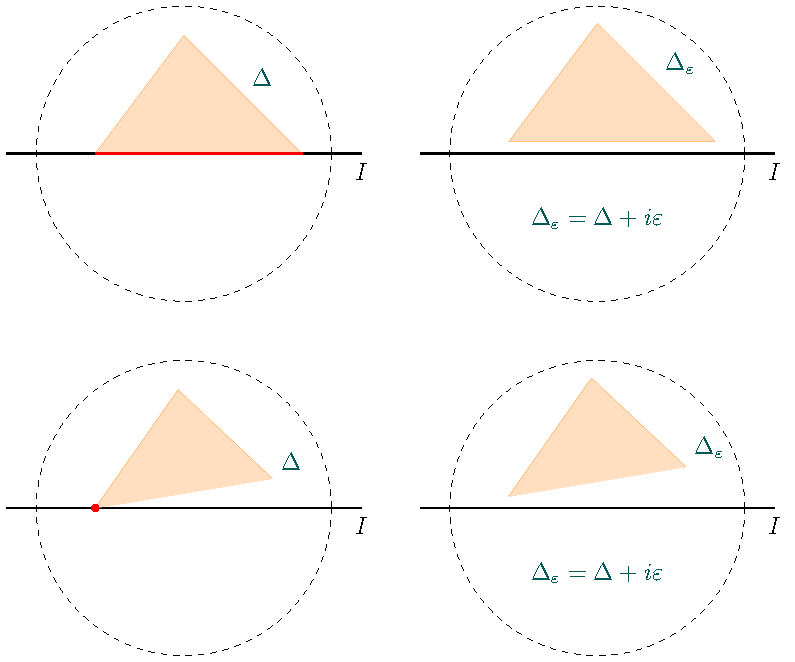
\includegraphics[width=0.8\textwidth]{%
                Figuras/casos 1 e 2 schwarz.pdf
            }
            \caption{Caso 1 (em cima) e 2 (abaixo) da Parte I da demonstração.}
        \end{figure}
        %
        Em ambos, temos
        %
        \begin{equation*}
            \int_{\Delta_{\e}} f(z)\, dz = 0,
        \end{equation*}
        %
        já que $\Delta_{\e}$ está inteiramente contido em $\Omega^+$.
        
        Daí, se $\y:[0,1]\to\C$ é uma parametrização de $\Delta$ então
        $\y_{\e}:[0,1]\to\C$ dada por 
        $\y_{\e}(t) = \y(t) + i\e$ é uma parametrização de
        $\Delta_{\e}$. Portanto,
        %
        \begin{align*}
            0 \equiv \int_{\Delta_{\e}} f(z)\, dz 
            &= \int_0^1 f(\y_{\e}(t))\y_{\e}'(t)\, dt \\
            &= \int_0^1 f(\y(t) + i\e)(\y(t) + i\e)'\, dt \\
            &= \int_0^1 f(\y(t) + i\e)\y'(t)\, dt.
        \end{align*}
        %
        Logo, 
        %
        \begin{equation*}
            \int_0^1 f(\y(t) + i\e)\y'(t)\, dt = 0
        \end{equation*}
        %
        e, daí,
        %
        \begin{align*}
            \lim_{\e\to 0} \int_0^1 f(\y(t) + i\e)\y'(t)\, dt = 0
        \end{align*}
        %
        que, pelo teorema da convergência dominada, pode ser escrito como
        %
        \begin{equation*}
            \int_0^1 \lim_{\e}f(\y(t) + i\e)\y'(t)\, dt = 0,
        \end{equation*}
        %
        ou seja,
        %
        \begin{equation*}
            \int_{\Delta} f(z)\, dz \equiv \int_0^1 f(\y(t))\y'(t)\, dt = 0
        \end{equation*}
        %
        \paragraph{Parte II:} $\Delta$ tem duas arestas interceptando $I$. Nesse caso, o interior
        de $\Delta$ intercepta $I$ e podemos reduzir esse caso a um dos anteriores se escrevermos 
        $\Delta$ como união de triângulos que têm um lado ou um vértice sobre $I$ da seguinte forma:
        %
        \begin{itemize}
            \item três triângulos como na Parte I no caso de $I$ interceptar $\Delta$
            em duas arestas;
            \item dois triângulos como na Parte II no caso de $I$ interceptar $\Delta$
            em uma aresta e um vértice.
        \end{itemize}
        %
        Os diagramas abaixo ilustram as situações.
        %
        \begin{figure}[H]\centering
            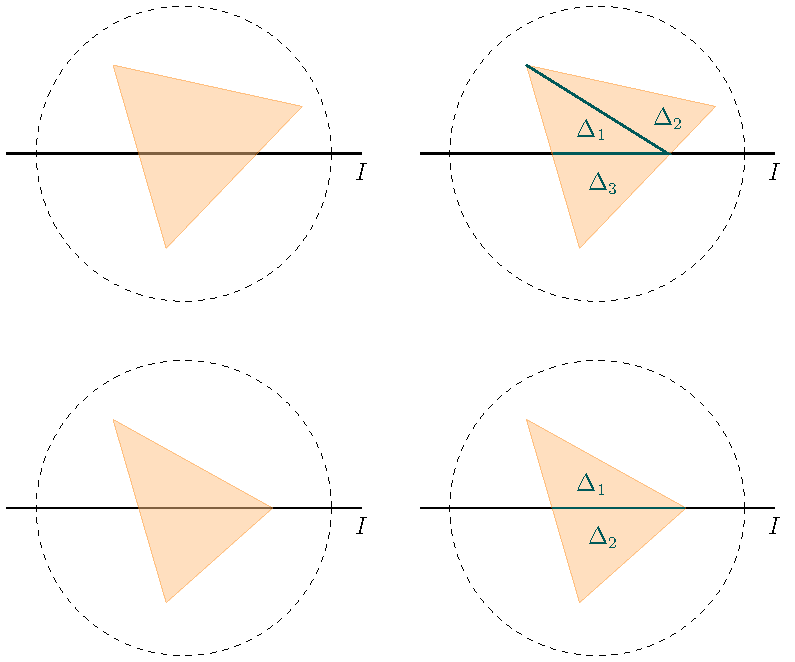
\includegraphics[width=0.8\textwidth]{
                Figuras/slide 16 aula 6.pdf
            }
            \caption{As duas possibilidades da Parte II da demonstração.}
        \end{figure}
        %
        Portanto, pelo Teorema de Morera segue que $f$ é holomorfa em $D$, como desejado.
    \end{proof}
    
    Podemos agora enunciar o princípio da reflexão, usando a mesma notação acima.
    
    \begin{teorema}[Princípio da Reflexão de Schwarz]
    \label{teo-reflexao-schwarz}
        Seja $\omega\subseteq\C$ um domínio simétrico e
        suponha que $f$ é uma função holomorfa em $\Omega^+$ que se estende 
        continuamente para $I$ e tal que $f$ toma valores reais em $I$. 
        Então existe uma função $F$ holomorfa em todo o $\Omega$ tal que
        $F\big|_{\Omega^+} = f$.
    \end{teorema}
        
    \begin{proof}
        A ideia é definir $F$ por
        %
        \begin{equation*}
            F(z) =
            %
            \begin{cases}
                f(z), & z \in \Omega^+ \\
                f(z), & z \in I \\
                \overline{f(\overline{z})}, & z\in\Omega^-   
            \end{cases}
            %
        \end{equation*}
        %
        Note que se tomarmos $f^+ \equiv f$ e $f^- \equiv \overline{f(\overline{z})}$, 
        em acordo com o princípio da simetria, temos que para qualquer $z_0\in I$
        %
        \begin{align*}
            \lim_{\substack{ z\to z_0 \\ \Im(z) > 0 }} f^+(z) 
            = 
            \overline{f(z_0)}
            =
            \overline{\lim_{\substack{ z\to z_0 \\ \Im(z) > 0 }} f(z)}
            =
            \lim_{\substack{ z\to z_0 \\ \Im(z) < 0 }} \overline{f(\overline{z})}
            =
            \lim_{\substack{ z\to z_0 \\ \Im(z) < 0 }} f^-(z),
        \end{align*}
        %
        ou seja, $f^+(z_0) = f^-(z_0)$ para todo $z_0\in I$. Portanto, mostrando que 
        $F$ é holomorfa em $\Omega^-$ poderemos usar o princípio da simetria para 
        concluir a holomorficidade de $F$ em todo $\Omega$.
        
        Sejam $z, z_0\in\Omega^-$ então $\overline{z}, \overline{z_0}\in\Omega^+$. 
        Desta forma, temos que
        %
        \begin{equation*}
            F(z) 
            = 
            \overline{f(\overline{z})} 
            =
            \overline{ \sum_{n=0}^{\infty}a_n(\overline{z} - \overline{z_0})^n }
            =
            \sum_{n=0}^{\infty}\overline{a_n}(z-z_0)^n,
        \end{equation*}
        %
        onde a segunda igualdade vale para todo 
        $\overline{z}\in D(\overline{z_0}, R_{\overline{z_0}}(f))$.
        
        Ora, uma vez que para todo $z\in D(z_0, R_{\overline{z_0}}(f))$ temos
        $\overline{z}\in D(\overline{z_0}, R_{\overline{z_0}}(f))$, segue da equação acima
        que $R_{z_0}(F)\geq R_{\overline{z_0}}(f)$ e, portanto, $F$ é holomorfa em
        $D(z_0, R_{z_0}(F))$.
    \end{proof}
%

\section{O teorema da aproximação de Runge}
\label{sec:aprox-runge}

    Nesta seção, tratamos do Teorema da aproximação de Runge, que é, num certo sentido, uma generalização do Teorema de Weierstrass enunciado abaixo.
    
    \begin{teorema}[Weierstrass]
    \label{teo:aprox-weierstrass}
        Seja $f:[a,b] \to \R$ uma função contínua. Existe uma sequência $\{p_n\}_{n\in\N}$ 
        de polinômios tal que $p_n \xrightarrow[n\to\infty]{\text{unif.}} f$.
    \end{teorema}
    
    Convergência uniforme significa que, dado qualquer $\e > 0$, existe $N \in \N$ 
    tal que 
    %
    \begin{equation*}
        n \geq N \implies \sup \{|f(x) - p_n(x)| : x \in [a,b] \} < \e.
    \end{equation*}
    %
    Este teorema mostra que podemos aproximar, por polinômios, uma função contínua qualquer 
    definida num intervalo fechado de uma forma global. Além disso, esta aproximação é uniforme, 
    ou seja, escolhido qualquer $\e > 0$, conseguimos encontrar um polinômio $p_n$ 
    tal que $f(x)$ está $\e-$próximo de $p_n(x)$ para todo $x$ em $[a,b]$. 
    Se não fosse uniforme, poderia ocorrer que, para cada $\e > 0$, 
    teríamos que encontrar um polinômio distinto para que a aproximação fosse boa o suficiente.
    
    No plano complexo, podemos aproximar (localmente) uma função holomorfa pelas somas parciais 
    de sua série de Taylor. O Teorema de Runge faz a aproximação (global) de funções holomorfas 
    num compacto por funções racionais. Para que a aproximação por polinômios seja possível, 
    é necessária uma hipótese adicional. Além disso, esse teorema é, em grande parte, 
    consequência da fórmula integral de Cauchy, como veremos na demonstração.
    %
    \begin{teorema}[Runge]
    \label{TR}
        O teorema consiste de dois pontos:
        \begin{enumerate}
            \item Qualquer função holomorfa definida em uma vizinhança de um compacto $K$ 
            pode ser aproximada uniformemente em $K$ por funções racionais cujas singularidades 
            estão em $K^c$.
            \item Se $K^c$ é conexo, qualquer função holomorfa em uma vizinhança aberta de $K$ 
            pode ser aproximada em $K$ por polinômios.
        \end{enumerate}
    \end{teorema}
    %
    A prova deste teorema será consequência de três lemas que provaremos a seguir.
    %
    \begin{lema}
    \label{LR1}
        Seja $f$ uma função holomorfa definida no aberto $\Omega$ e seja $K \subseteq \Omega$ 
        um compacto. Existem finitos segmentos de reta $\y_1, \dots, \y_N$ em 
        $\Omega - K$ tais que
        %
        \begin{equation*}
        f(z) 
        = 
        \sum^{N}_{j=1}\frac{1}{2 \pi i}\int_{\y_j}\frac{f(w)}{w-z} \, dw  \, , \forall z \in K.
        \end{equation*}
        %
    \end{lema}
    %
    \begin{proof}
        Seja $d = c \cdot d(K, \Omega^c)$, onde $0 < c < 1/\sqrt{2}$ e
        %
        \begin{equation*}
        d(K, \Omega^c) = \inf \{d(z,w) : z \in K, w \in \Omega^c\}.
        \end{equation*}
        %
        Considere um reticulado de quadrados com lados de medida $d$ e paralelos aos eixos 
        coordenados (veja Figura \ref{fig:reticulado runge}). Seja $\mathcal{Q} = \{Q_1, \dots, Q_M\}$ o conjunto 
        dos quadrados unidos aos seus interiores que interceptam o conjunto $K$ (finito pois
        $K$ é compacto). Vamos chamar, daqui em diante, os elementos de $\mathcal{Q}$ de quadrados.
        %
        \begin{figure}[H]\centering
            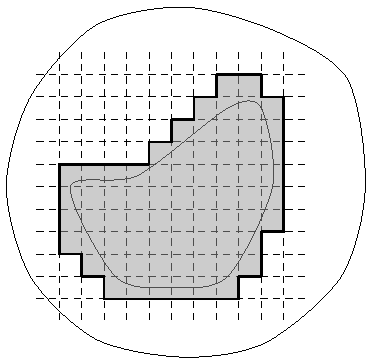
\includegraphics{
                Figuras/reticulado-para-Runge.pdf
            }
        	\caption{A união dos caminhos $\y_j$ está negritada.}
        	\label{fig:reticulado runge}
        \end{figure}
        %
        Sejam $\y_j$, com $j \in \{1, \dots, N\}$, os lados dos quadrados em $\mathcal{Q}$ 
        que não são lados de quadrados adjacentes de $\mathcal{Q}$. Pela escolha de $d$, temos 
        que $d\sqrt{2}$ é a medida da diagonal dos quadrados e é menor que $d(K, \Omega^c)$, 
        logo $\y_j\subset\Omega$ para todo $j$.
        
        Se $z$ está em $K$ e $z \in Q_m - \partial Q_m$, então, pela fórmula integral de Cauchy,
        %
        \begin{equation*}
            \frac{1}{2 \pi i}\int_{\partial Q_m}\frac{f(w)}{w-z}\, dw 
            = 
            \begin{cases}
                f(z), &m = j \\
                0, &m \neq j.
            \end{cases}
        \end{equation*}
        %
        Portanto, para todo $z\in K$ que não está no bordo de nenhum quadrado de $\mathcal{Q}$, 
        temos
        %
        \begin{equation*}
            f(z) = \sum^{M}_{m=1}\frac{1}{2 \pi i}\int_{\partial Q_m}\frac{f(w)}{w-z}\,dw.
        \end{equation*}
        %
        Como $f$ é contínua em $K$, para $z_0 \in K \cap \partial Q_j$ para algum $j$, temos
        %
        \begin{align*}
            f(z_0) &= \lim_{\substack{z \to z_0 \\ z\in K}} f(z) \\
                   &= \lim_{\substack{z \to z_0 \\ z\in K}} 
                   \frac{1}{2 \pi i}\int_{\partial Q_m}\frac{f(w)}{w-z}\,dw \\
                   &= \frac{1}{2 \pi i}\int_{\partial Q_m}\frac{f(w)}{w-z_0}\,dw,
        \end{align*}
        %
        Portanto, está demonstrado o lema.
    \end{proof}
    %
    \begin{lema}
    \label{LR2}
        Para qualquer segmento de reta contido em $\Omega - K$, existe uma sequência 
        de funções racionais com singularidades em $\y$ que aproxima
        %
        \begin{equation*}
        \int_\y \frac{f(w)}{w-z}\,dw
        \end{equation*}
        %
        uniformemente em $K$.
    \end{lema}
    %
    \begin{proof}
        Seja $\y : [0,1] \to \C$ um segmento de reta conforme o teorema e denote
        %
        \begin{equation*}
            F(z,t) = \frac{f(\y(t))}{\y(t) - z}\y'(t).
        \end{equation*}
        %
        Note que $F$ é uma função contínua em $K \times [0,1]$ e que
        %
        \begin{equation*}
            \int_\y \frac{f(w)}{w-z}\,dw = \int_{0}^{1}F(z,t)\,dt.
        \end{equation*}
        %
        Fixado $z \in K$ e dado $\e > 0$, existe um $\delta_z > 0$ tal que
        %
        \begin{equation}
        \label{ER1}
            |t_1 - t_2| < \delta_z \implies |F(z,t_1) - F(z,t_2)| < \e
        \end{equation}
        %
        Pela continuidade de $F$, existe um $\eta_z > 0$ tal que, para $z_1$ satisfazendo 
        $|z-z_1| < \eta_z$, ainda vale \eqref{ER1}. Como $K$ é compacto, podemos escolher 
        um $\delta > 0$ tal que
        %
        \begin{equation}
        \label{ER2}
            |t_1 - t_2| < \delta \implies \sup \{|F(z,t_1) - F(z,t_2)| : z \in K\} < \e.   
        \end{equation}
        %
        Podemos escrever a integral de $F(z,t)$ de $0$ a $1$ como o limite de uma soma de Riemann 
        (que converge uniformemente):
        %
        \begin{equation*}
            \int_{0}^{1}F(z,t) \, dt = \lim_{n \to \infty}\frac{1}{n}\sum_{j=1}^{n}F(z,t_j),
        \end{equation*}
        %
        onde cada $F(z,t_j)$ é uma função racional. Denote
        %
        \begin{equation*}
            g(z) = \int_{0}^{1}F(z,t) \, dt \, ,  \ \ \ \ g_n(z) = \frac{1}{n}\sum_{j=1}^{n}F(z,t_j).
        \end{equation*}
        %
        Usando as considerações anteriores, temos que 
        \begin{align*}
            |g(z) - g_n(z)| 
            &\leq 
            \sum_{k=1}^{n}\frac{1}{n}\left|\int_{\frac{k-1}{n}}^{\frac{k}{n}}F(z,k/n) - F(z,n) \, dt \right| \\
            &\leq \sum_{k=1}^{n}\frac{1}{n}\int_{\frac{k-1}{n}}^{\frac{k}{n}}|F(z,k/n) - F(z,n)| \, dt
            \to 0,
        \end{align*}
        onde usamos \eqref{ER2}. Observe que $g(z)$ é a expressão que queríamos aproximar
        (uniformemente) por funções racionais, então o Lema está demonstrado.
    \end{proof}
    %
    \\ \\
    
    Para ilustrar a necessidade da hipótese da conexidade de $K^c$, damos um exemplo. 
    Considere a função $f: \C^* \to \C$ dada pela regra $z \mapsto 1/z$ e o compacto 
    $\partial \D$, o bordo do disco unitário  $\D$. Vamos mostrar que $f$ não
    pode ser aproximada por polinômios em $\partial D$, mesmo esse conjunto sendo compacto.
    Observe ainda que o seu complementar é um conjunto desconexo.
    
    Pelo Teorema dos Resíduos, por exemplo, sabemos que
    %
    \begin{equation*}
        \int_{\partial \D}f(z) \, dz = 2 \pi i.
    \end{equation*}
    %
    Suponha, por contradição, que $f$ tenha uma aproximação uniforme por polinômios em 
    $\partial \D$. Então existe uma sequência $\{p_n\}$ de polinômios tal que, 
    dado $\e > 0$, existe $N \in \N$ tal que
    %
    \begin{equation*}
        n \geq N \implies \sup \{|f(z) - p_n(z)|: z \in \partial \D\} < \e.
    \end{equation*}
    %
    Além disso, a integral de qualquer polinômio ao redor de uma curva simples e fechada é sempre
    igual a zero, pois polinômios são funções inteiras. Segue que
    %
    \begin{align*}
        \left|\int_{\partial \D} f(z) \, dz\right| 
        &= \left|\int_{\partial \D} f(z) \, dz - \int_{\partial \D} p_n(z) \, dz\right| \\
        &= \left|\int_{\partial \D} f(z) - p_n(z)\, dz\right| \\
        &\leq \int_{\partial \D}|f(z) - p_n(z)| \, dz \xrightarrow{n\to\infty} 0,
    \end{align*}
    %
    Isto é uma clara contradição e mostra a importância da hipótese de que $K^c$ seja {\bf conexo}.
    %
    \begin{lema}
    \label{LR3}
        Se $K^c$ é conexo e $z_0 \not \in K$, então $\displaystyle{\frac{1}{z-z_0}}$ 
        pode ser aproximado em $K$ por polinômios.
    \end{lema}
    %
    \begin{proof}
        Seja $D$ um disco com centro na origem que contém $K$ (tal disco existe porque 
        $K$ é compacto). Sendo $z_1 \not \in D$, podemos aproximar $1/(z-z_1)$ por polinômios
        definidos em $K$. De fato, veja que
        %
        \begin{equation*}
        \frac{1}{z-z_1}
        =
        \frac{-1}{z_1}\cdot\frac{1}{1-\frac{z}{z_1}} = - \sum_{n=1}^{\infty}\frac{z^n}{z_1^{n+1}}.
        \end{equation*}
        %
        Esta série converge sempre que $|z| < |z_1|$ e, em particular, converge uniformemente 
        para todo $z \in K$. As suas somas parciais, então, são uma aproximação uniforme, 
        como afirmado. Como consequência disso, podemos aproximar da mesma forma qualquer 
        potência $1/(z-z_1)^k$.
        
        Como $K^c$ é conexo, existe uma curva $\y : [0,1] \to \C$ inteiramente contida em 
        $K^c$ tal que $\y(0) = z_0$ e $\y(1) =  z_1$. Defina $\rho = \frac{1}{2}d(K,\y)$;
        devemos ter $\rho > 0$ pois ambos $K$ e $\y$ são compactos. 
        Seja $\{w_0, w_1, \dots, w_l\}$ uma sequência finita de pontos em $\y$ com $w_0 = z_0$,
        $w_l = z_1$ e $|w_j - w_{j+1}| < \rho$ para $0 \leq j < l$. Sendo $w = w_j$ para algum $j$,
        temos que se $w'$ satisfaz $|w - w'| < \rho$, podemos aproximar $\frac{1}{z-w}$ 
        por polinômios em $\frac{1}{z-w'}$. De fato, basta notar que
        %
        \begin{align*}
            \frac{1}{z-w} &= \frac{1}{z - w' + w' - w}\\
                          &= \frac{1}{z-w'}\frac{1}{1 - \frac{w - w'}{z - w'}}\\
                          &= \sum_{n = 0}^{\infty}\frac{(w-w')^n}{(z-w')^{n+1}},
        \end{align*}
        %
        onde a convergência é uniforme para $|w-w'| < |z-w'|$. Isto acontece para todo 
        $z \in K$, pois $|z-w'|> \rho$.
        
        Fazendo isto repetidamente para os pontos da sequência finita $\{w_j\}$, vemos que 
        $1/(z-z_0)$ pode ser aproximado por polinômios em $1/(z-z_1)$ que, por sua vez, pode 
        ser aproximado por polinômios em $K$.
    \end{proof}
    %
    \\
    
    O Lema \ref{LR1} nos dá uma expressão para $f$ em $K$ em termos de uma certa soma em 
    que vemos claramente a fórmula integral de Cauchy. O Lema \ref{LR2} mostra que cada parcela 
    dessa soma pode ser aproximada por funções racionais de forma uniforme; além disso, as
    singularidades dessas funções estão fora de $K$. Isto demonstra o item 1 do Teorema de Runge. 
    Em essência, o Lema \ref{LR3} implica o segundo item do Teorema porque os denominadores das
    funções racionais do item 1 poderão ser aproximados por polinômios quando aplicamos a hipótese
    de conexidade de $K^c$.
    
\section{Integrais Complexas Impróprias e a Transformada de Fourier}
\label{sec:integrais-e-transf-fourier}

    Neste seção, começamos a tratar da transformada de Fourier. Para tanto, é necessário
    primeiro definir de maneira mais rigorosa a integral complexa e a integral imprópria e,
    para este objetivo, tratamos brevemente da medida de Lebesgue. Buscamos fazer o máximo da
    teoria no âmbito da integração de Riemann, mas em alguns enunciados são necessárias hipóteses
    que utilizam a medida de Lebesgue.
    
    \subsection{Uma brevíssima introdução à medida de Lebesgue}
        %
        \begin{definicao}
        \label{def-medida-lebesgue}
            A medida de Lebesgue é a correspondência
            %
            \begin{equation*}
                \Leb: \mathcal{A}\subset\mathcal{P}(\R) \to [0, +\infty] \subseteq\overline{\R} 
                = \R\cup\{-\infty, +\infty\},
            \end{equation*}
            %
            sendo $\mathcal{A}$ uma $\sigma$-álgebra adequada\footnote{Não vamos falar da
            estrutura exata dessa $\sigma$-álgebra; basta saber que ela é maior que os borelianos
            mas menor que o conjunto das partes.} e $\overline{\R}$ a reta real estendida, tal que
            %
            \begin{equation*}
                \Leb(A) = \inf_{\mathcal{C}} \sum_{n\in\N} (b_n - a_n), \, \forall A\in\mathcal{A},
            \end{equation*}
            %
            onde $\mathcal{C}$ é a família de coberturas abertas $\mathscr{C}$ de $A$ por intervalos
            disjuntos, i.e.,
            %
            \begin{equation*}
                \mathscr{C} = \bigcup_{n\in\N} I_n, \text{ com } I_n = (a_n, b_n)\subseteq\R
                \text{ e } I_j\cap I_k = \varnothing, j\neq k.
            \end{equation*}
            %
        \end{definicao}
        %
        Com essa definição, temos, por exemplo, que
        %
        \begin{align*}
            \Leb([a,b]) = b-a = \Leb((a,b))
        \end{align*}
        %
        e também que a medida de Lebesgue de uma união disjunta é a soma das medidas, ou seja,
        %
        \begin{equation*}
            \Leb\left( \bigsqcup_k I_k \right) = \sum_k \Leb(I_k).
        \end{equation*}
        %
        Um tratamento mais aprofundado e no contexto de Teoria da Probabilidade pode ser
        encontrado \href{https://github.com/leandro-mat/Notas-PTM/blob/master/notas.pdf}{aqui}.
        Antes de rumar para a integração, vamos apenas mostrar uma propriedade interessante
        da medida de Lebesgue: todo conjunto enumerável tem medida nula.
        %
        \begin{proposicao}
        \label{enumeravel-medida-nula}
            $\Leb(\mathcal{Q}) = 0$ para todo $\mathcal{Q}$ enumerável.
        \end{proposicao}
        %
        \begin{proof}
            Seja $\{ p_1, p_2, \dots, p_n, \dots \}$ uma enumeração de $\mathcal{Q}$ e considere
            a cobertura de $\mathcal{Q}$ pelos intervalos
            %
            \begin{equation*}
                I_n = \left(p_n - \frac{\e}{2^n}, p_n + \frac{\e}{2^n} \right),
            \end{equation*}
            %
            sendo $\e>0$ qualquer. Daí, temos
            %
            \begin{align*}
                \Leb(\mathcal{Q}) &\leq \sum_{n\in\N} \Leb(I_n) \\
                                  &= \sum_{n\in\N} \frac{2\e}{2^n} \\
                                  &= 2\e\sum_{n\in\N} \frac{1}{2^n} \\
                                  &= 2\e.
            \end{align*}
            %
            Como $\e$ é qualquer, segue que $\Leb(\mathcal{Q}) = 0$.
        \end{proof}
        %
        \begin{corolario}
            $\Leb(\Q) = 0$.
        \end{corolario}
        %
        Mostramos que todo conjunto enumerável tem medida de Lebesgue nula, mas a volta
        não vale! Dito de outro modo, existem conjuntos não-enumeráveis com medida nula.
        Um exemplo clássico é o conjunto de Cantor, $\mathbf{C}$.
        %
        \begin{proposicao}
        \label{cantor-medida-nula}
            O conjunto de Cantor, $\mathbf{C}$, tem medida de Lebesgue nula.
        \end{proposicao}
        %
        \begin{proof}
            Para mostrar essa fato, vamos olhar para os ``pedaços'' removidos do conjunto de
            Cantor e usar o fato de que $\Leb([0,1]) = 1$. No passo $N$ da construção de 
            $\mathbf{C}$, removemos um comprimento de
            %
            \begin{equation*}
                \sum_{n=1}^N \frac{2^{n-1}}{3^n}=\frac{1}{2}\sum_{n=1}^N \left(\frac{2}{3}\right)^n
                \xrightarrow{N\to +\infty} \frac{1}{2}\cdot\frac{2/3}{1/3} = 1.
            \end{equation*}
            %
            Dado $\e>0$, existe $N_0\in N$ tal que
            %
            \begin{equation*}
                \frac{1}{2}\sum_{n=1}^{N_0} \left(\frac{2}{3}\right)^n > 1 - \e.
            \end{equation*}
            %
            Seja $\{I_k\}$ a família de intervalos que corresponde a essa soma. Ora, então
            $\left( \bigcup_k I_k \right)^c$ é uma cobertura de $\mathbf{C}$ com soma
            dos comprimentos menor que $\e$. Da arbitrariedade de $\e$, segue que
            $\Leb(\mathbf{C}) = 0$.
        \end{proof}
        %
        
    \subsection{Integrais Impróprias e o Valor Principal de Cauchy} %colocar o Lema Técnico aqui?
        %
        Se $f:[a,b]\to\R$ é uma função limitada tal que o seu conjunto de pontos de descontinuidade
        tem medida de Lebesgue nula, então existe a integral de Riemann de $f$, ou seja, existe
        o limite
        %
        \begin{equation*}
            \lim_{n\to\infty} \frac{b-a}{n}\sum_{j=1}^n f(x_j^*) = \int_a^b f(x) \, dx,
        \end{equation*}
        %
        sendo $x_j^*$ o ponto médio do intervalo 
        $\displaystyle{ \left[ a + \frac{b-a}{n}(j-1), a + \frac{b-a}{n}j \right] }$.
        
        A discussão feita acima sobre a medida de Lebesgue nos permite ver que impor a condição
        de que as descontinuidades de $f$ tenha medida nula não é, de modo algum, restritiva demais:
        funções com os mais diferentes tipos de conjuntos de descontinuidade estão nessa classe.
        %
        \begin{definicao}
        \label{def-riemann-integravel}
            Seja $f:\R\to\R$ uma função com conjunto de descontinuidades de medida nula. Suponha
            que $f$ é limitada em cada compacto $[a,b]\subseteq\R$, isto é, tal que
            %
            \begin{equation*}
                \sup_{x\in [a,b]} |f(x)| < +\infty.
            \end{equation*}
            %
            Se existir
            %
            \begin{equation*}
                \lim_{\substack{b\to +\infty \\ a\to -\infty}} \int_a^b f(x) \, dx 
                \equiv \int_{\R} f(x) \, dx \in\overline{\R},
            \end{equation*}
            %
            dizemos que $f$ é Riemann integrável em $\R$.
        \end{definicao}
        %
        Aqui é conveniente observar o seguinte: por vezes, é dito apenas ``integrável'' ao invés
        de ``Riemann integrável'' ou ``Lebesgue integrável'' (que não definimos). É importante
        saber a qual dessas duas o contexto se refere, pois no caso de Riemann integrável queremos
        1) saber se o limite acima existe e 2) quanto ele vale (podendo ser infinito); por outro
        lado, no caso de Lebesgue integrável queremos saber apenas se o limite acima é finito,
        pois ele sempre existe nesse segundo contexto. Aqui, a menos que dito o contrário,
        estaremos nos referindo à integrabilidade de Riemann.
        
        Ademais, vamos reservar o símbolo
        %
        \begin{equation*}
            \int_{\R} f(x) \, dx
        \end{equation*}
        %
        para a integral acima, em que os limites superior e inferior da integral definida
        convergem para infinito a qualquer taxa.
        %
        \begin{definicao}
        \label{def-valor-principal}
            O Valor Principal de Cauchy de uma função $f:\R\to\R$, quando existe, é dado pelo limite
            %
            \begin{equation*}
                \lim_{a\to +\infty} \int_{-a}^a f(x) \, dx 
                \equiv \text{VP}\left( \int_{-\infty}^{\infty} f(x) \, dx \right)
                \equiv \int_{-\infty}^{\infty} f(x) \, dx
            \end{equation*}
            %
        \end{definicao}
        %
        Fica evidente desta definição que se $f:\R\to\R$ é Riemann integrável, então
        %
        \begin{equation*}
            \int_{\R} f(x) \, dx = \int_{-\infty}^{\infty} f(x) \, dx,
        \end{equation*}
        %
        ou seja, a integral é dada pelo Valor Principal de Cauchy. Isto nos permite trabalhar de
        maneira mais fácil: se sabemos que o limite da Definição \ref{def-riemann-integravel} 
        existe, podemos calculá-lo utilizando o limite da Definição \ref{def-valor-principal}, 
        que é muito mais facilmente tratável do que o primeiro.
        
        Observamos que nem toda função que tem um valor principal de Cauchy é Riemann integrável. Considere
        %
        \begin{equation*}
            \lim_{\substack{b\to +\infty \\ a\to -\infty}} \int_a^b \sen{x} \, dx. 
        \end{equation*}
        %
        Se escolhemos taxas particulares $b = (2n+1)\pi/2$ e $a = 2n\pi$ vemos que essa integral converge a $1$. 
        Se $b = 2n\pi$ e $a = (2n+1)\pi/2$, então ela converge a $-1$. Portanto, este limite não existe e 
        $\sen{x}$ não é Riemann integrável. No entanto, se $a = b = r$, i.e., se consideramos a mesma taxa, 
        a integral resulta em
        %
        \begin{equation*}
            \lim_{r \to \infty} - \cos r + \cos(-r) = 0,
        \end{equation*}
        %
        pois $\cos r = \cos(-r)$. Portanto, $\sen{x}$ tem um valor principal de Cauchy.
        %
    \subsection{Integrais de Funções Complexas}
        %
        Vamos trabalhar com dois tipos de integrais de funções que tomam valores em $\C$:
        %
        \begin{enumerate}
            \item integrar $\widetilde{f}:[a,b]\to\C$, com 
            $\widetilde{f}(t) = \widetilde{f_1}(t) + i\widetilde{f_2}(t)$;
            %
            \item integrar $f:U\to\C$ ao longo de um caminho $\y:[a,b]\to\C$ suave por
            partes tal que $\y(t)\in U, \forall t\in [a,b]$.
        \end{enumerate}
        %
        Para as funções do primeiro tipo, definimos a integral motivados pela definição da integral
        de Riemann, utilizando a ideia de média.
        %
        \begin{definicao}
        \label{def-integral-complexa-tipo-1}
            Seja $f:[a,b]\to\C$ uma função complexa dada por $f(t) = f_1(t) + if_2(t)$, sendo
            $f_1, f_2$ funções que tomam valores em $\R$. Supondo $f_1$ e $f_2$ Riemann
            integráveis em $[a,b]$, definimos
            %
            \begin{equation*}
                \int_a^b f(t) \, dt = \lim_{n\to\infty}\left(\frac{b-a}{n}\sum_{j=1}^n f(t_j^*)\right),
            \end{equation*}
            %
            com $t_j^*$ o ponto médio do intervalo 
            $\displaystyle{ \left[ a + \frac{b-a}{n}(j-1), a + \frac{b-a}{n}j \right] }$.
        \end{definicao}
        %
        Já que estamos assumindo $f_1, f_2$ Riemann integráveis em $[a,b]$, temos que
        %
        \begin{align*}
            \int_a^b f(t) \, dt &= \lim_{n\to\infty}\left(\frac{b-a}{n}\sum_{j=1}^n f(t_j^*)\right) \\
                                &= \lim_{n\to\infty}\left(\frac{b-a}{n}\sum_{j=1}^n [f_1(t_j^*) 
                                + if_2(t_j^*)] \right) \\
                                &= \lim_{n\to\infty}\left(\frac{b-a}{n}\sum_{j=1}^n f_1(t_j^*)\right)
                                + i\lim_{n\to\infty}\left(\frac{b-a}{n}\sum_{j=1}^n f_2(t_j^*)\right) \\
                                &= \int_a^b f_1(t) \, dt + i\int_a^b f_2(t) \, dt.
        \end{align*}
        %
        Isso nos mostra o porquê da ``definição razoável'' da integral complexa no primeiro caso
        ser o número complexo formado pelas integrais de cada uma das partes: a definição através
        da mesma ideia da integral de Riemann.
        %
        \begin{definicao}
        \label{def-integral-complexa-impropria-tipo-1}
            Seja $f:\R\to\C$ uma função complexa tal que suas partes real e imaginária,
            $f_1\equiv\Re(f)$ e $f_2\equiv\Im(f)$, são funções Riemann integráveis em $\R$.
            Então, definimos a integral de $f$ em $\R$ por
            %
            \begin{equation*}
                \int_{\R} f(t) \, dt=\lim_{\substack{b\to +\infty \\ a\to -\infty}}\int_a^b f(t) \, dt
                                    = \int_{\R} f_1(t) \, dt + i\int_{\R} f_2(t) \, dt
            \end{equation*}
            %
        \end{definicao}
        %
        De maneira análoga definimos o Valor Principal de Cauchy:
        %
        \begin{definicao}
        \label{def-valor-principal-integral-complexa-tipo-1}
            O Valor Principal de Cauchy de uma função $f:\R\to\C$, tal que suas partes 
            real e imaginária, $f_1\equiv\Re(f)$ e $f_2\equiv\Im(f)$, são funções Riemann 
            integráveis em $\R$ é
            %
            \begin{equation*}
                \lim_{a\to +\infty} \int_{-a}^a f(t) \, dt
                \equiv \text{VP}\left( \int_{-\infty}^{\infty} f(t) \, dt \right)
                \equiv \int_{-\infty}^{\infty} f(t) \, dt
                = \int_{-\infty}^{\infty} f_1(t) \, dt + i\int_{-\infty}^{\infty} f_2(t) \, dt
            \end{equation*}
            %
        \end{definicao}
        %
        Os resultados que vamos apresentar mais à frente são válidos para funções Riemann
        integráveis em $\R$ e vamos mostrar que a classe de funções que será de nosso interesse
        satisfaz essa propriedade.
        
        Para funções do segundo tipo, isto é, funções $f:U\subseteq\C\to\C$, vamos utilizar o
        conceito de integral de linha. Portanto, precisamos fixar um caminho suave por partes
        $\y:[0,1]\to\C$ (normalizado). Assim, definimos
        %
        \begin{equation}
        \label{def-integral-complexa-tipo-2}
            \int_{\y} f(z) \, dz \equiv \int_0^1 f(\y(t))\y'(t) \, dt,
        \end{equation}
        %
        onde a integral no lado direito é a integral de $g:[0,1]\to\C$ dada por 
        $g(t) = f(\y(t))\y'(t), \forall t\in [0,1]$.
        
        Para que \eqref{def-integral-complexa-tipo-2} esteja bem definida, precisamos que
        $g$ seja Riemann integrável em $[a,b]$ e que a integral independe da parametrização
        de $\y$.
        
        De maneira análoga, se $\y:\R\to\C$ é um caminho suave com $\y(\R)$ um
        subconjunto do domínio de $f$, definimos
        %
        \begin{align*}
            \int_{\y} f(z) \, dz \equiv \int_{\R} f(\y(t))\y'(t) \, dt
                                     \equiv \lim_{\substack{b\to +\infty \\ a\to -\infty}} 
                                     \int_a^b f(\y(t))\y'(t) \, dt,
        \end{align*}
        %
        desde que o último limite existe em $\overline{\C} = \C\cup\{\infty\}$. Intuitivamente,
        $\y:\R\to\C$ seria um caminho ``infinito''; entretanto, vamos reservar o termo ``caminho''
        para $\y:[0,1]\to\C$.
        
    \subsection{A Transformada de Fourier}
        %
        Se $f:\R\to\R$ é uma função satisfazendo certas condições de regularidade e decaimento,
        sua transformada de Fourier é definida por
        %
        \begin{equation}
        \label{def-transf-fourier}
            \widehat{f}(\xi) = \int_{-\infty}^{\infty} f(x) e^{-2\pi ix\xi} \, dx.
        \end{equation}
        %
        Veremos ainda que, quando existir, a inversa dessa transformada será dada por
        %
        \begin{equation*}
        \label{def-inv-trans-fourier}
            f(x) = \int_{-\infty}^{\infty} \widehat{f}(\xi) e^{2\pi ix\xi} \, d\xi.
        \end{equation*}
        %
        Vamos assumir que $f:\R\to\R$ admite uma extensão analítica a uma faixa horizontal contendo
        o eixo real e tendo decaimento moderado no infinito (vamos precisar mais à frente o quão
        moderado esse decaimento deve ser). Com isso, veremos mais à frente que essas hipóteses
        nos permitem concluir que
        %
        \begin{itemize}
            \item $\widehat{f}$ converge;
            %
            \item $\widehat{f}$ decai exponencialmente no infinito;
            %
            \item a inversa de $\widehat{f}$ existe e é dada como em \eqref{def-inv-trans-fourier}
            %
            \item vale a famosa fórmula da soma de Poisson:
            %
            \begin{equation}
            \label{def-soma-poisson}
                \sum_{n\in\Z} f(n) = \sum_{n\in\Z} \widehat{f}(n).
            \end{equation}
            %
        \end{itemize}
        %
        Como veremos, todos esses resultados são consequências da Fórmula Integral de Cauchy.
        
    \subsection{A classe \texorpdfstring{$\mathfrak{F}$}{F}}
        %
        Vamos, aqui, considerar uma classe de funções que é adequada aos nossos estudos, mas
        que não é a mais geral possível para se desenvolver a teoria de Fourier. Dito de outro
        modo, a nossa classe de funções com transformada de Fourier, $\mathfrak{F}$, pode ser
        ampliada.
        
        A construção de $\mathfrak{F}$ será feita em duas etapas.
        
        \paragraph{1ª etapa.} Defina, para cada $a>0$,
        %
        \begin{equation*}
            \mathfrak{F}_a = \left\{ f:U\subseteq\C\to\C \ | \ 
            f \text{ é holomorfa, } S_a\subseteq U \text{ e } f(\R)\subseteq\R \right\},
        \end{equation*}
        %
        sendo $S_a$ a faixa horizontal contendo o eixo real com largura $2a$. Vamos supor, ainda,
        que existe uma constante $A>0$ tal que
        %
        \begin{equation*}
            |f(x+iy)| \leq \frac{A}{1 + x^2}, \, \forall x\in\R, |y|<a.
        \end{equation*}
        %
        \begin{figure}[H]
				\centering 
				\begin{tikzpicture}
				\draw (-5,2)--(5,2);
				\draw (-5,-2)--(5,-2);
				\draw[-latex] (-5,0)--(5,0) node [at end,right]{$\Re$};
				\draw[-latex] (0,-3)--(0,3) node [at end,above]{$\Im$};
				\node [at={(0,2)}, above right]{$ia$};
				\node [at={(0,-2)}, below right]{$-ia$};
				\draw[red] (-5,1.2)--(5,1.2) node [at end,above]{$y=\Im(z)$};
				\node [at={(0,1.2)}, above left]{$y$};
				\end{tikzpicture}
			\end{figure}
        %
        Note que a constante $A$ é uniforme na reta $y = \Im(z)$, isto é, $A$ independe da 
        ``altura'' em que estamos na faixa.
        
        Vamos dar alguns exemplos de funções que satisfazem essas condições.
        %
        \begin{exemplo}
            Seja $f:\C\to\C$ dada por $f(z) = e^{-\pi z^2}$. Temos $f\in\mathfrak{F}_a, \forall a>0$.
            De fato, dado $a>0$, temos que
            %
            \begin{align*}
                |f(x+iy)| &= |\exp(-\pi(x+iy)^2)| \\
                          &= |\exp(-\pi(x^2-y^2+2ixy))| \\
                          &= \exp(-\pi x^2)\exp(\pi y^2) \\
                          &\leq \exp(-\pi x^2)\underbrace{\exp(\pi a^2)}_{\equiv A}.
            \end{align*}
            %
            Resta analisar $\exp(-\pi x^2)$. Expandindo em série de Taylor, temos
            %
            \begin{equation*}
                \exp(\pi x^2) = 1 + \pi x^2 + \frac{(\pi x^2)^2}{2!} + \frac{(\pi x^2)^3}{3!} + \cdots
                              \geq 1 + \pi x^2.
            \end{equation*}
            %
            Logo,
            %
            \begin{equation*}
                \frac{1}{\exp(\pi x^2)}\leq\frac{1}{1+\pi x^2}\leq\frac{1}{1+x^2},\forall x\in\R.
            \end{equation*}
            %
            Daí, segue que
            %
            \begin{align*}
                |f(x+iy)| \leq A\exp(-\pi x^2) \leq \frac{A}{1+x^2}
            \end{align*}
            %
            e, portanto, $f\in\mathfrak{F}_a, \forall a>0$.
        \end{exemplo}
        %
        \begin{exemplo}
            Dado $c>0$ fixo, temos que $f:\C\setminus\{\pm ic\}\to\C$ dada por
            %
            \begin{equation*}
                f(z) = \frac{1}{\pi}\cdot\frac{c}{c^2 + z^2}
            \end{equation*}
            %
            pertence a $\mathfrak{F}_a$ para todo $0 < a < c$\footnote{Essa $f$ pode parecer artificial,
            mas ela está relacionada ao núcleo de Poisson, que, por sua vez, tem relação com
            as soluções estacionárias do problema de Dirichlet do calor no semi-plano superior.}.
            
            De fato, note primeiramente que $|c^2+z^2| = |z-ic|\cdot |z+ic|$ é invariante por
            conjugação.
            %
            \begin{center}
                {\bf diagrama slide 24 Aula 8}
            \end{center}
            %
            Escolha $2c = d \gg a$ e seja $R_{a,d} = [-d,d]\times[-a,a]$.
            Considere a função $h$ dada por $h(z) = z^2 + c^2$. Ela é inteira, de modo que
            pelo Teorema do Módulo Máximo temos
            %
            \begin{equation*}
                \min_{z\in R_{a,d}} |h(z)| = \min_{z\in\partial R_{a,d}} |h(z)| = |a+c|\cdot|a-c|.
            \end{equation*}
            %
            Portanto, para todo $z\in R_{a,d}$ temos
            %
            \begin{align*}
                |f(z)| &= \frac{1}{2\pi}\cdot\frac{c}{|z^2 + c^2|} \\
                       &\leq \frac{1}{2\pi}\cdot\frac{c}{|a+c|\cdot|a-c|} \\
                       &= \frac{1}{2\pi}\cdot\frac{c}{|a+c|\cdot|a-c|}\cdot\frac{1+x^2}{1+x^2} \\
                       &\leq\frac{1}{2\pi}\cdot\frac{c(1+d^2)}{|a+c|\cdot|a-c|}\cdot\frac{1}{1+x^2}.
            \end{align*}
            %
            Agora, vaoms estimar $|f(z)|$ com $|z|\geq d = 2c$. Temos que
            %
            \begin{equation*}
                |z|\geq 2c \implies |z|^2 \geq 4c^2 \implies \frac{1}{4} \leq \frac{c^2}{|z|^2},
            \end{equation*}
            %
            donde, pela segunda desigualdade triangular, segue que
            %
            \begin{align*}
                \frac{3}{4} = \left|1 - \frac{c^2}{|z|^2}\right| \leq \left|1 + \frac{c^2}{z^2}\right|.
            \end{align*}
            %
            Ademais, se $x\geq 0$ é tal que $2c \leq x^2$, então
            %
            \begin{equation*}
                \frac{1}{x^2} = \frac{1+x^2}{x^2}\cdot\frac{1}{x^2+1}
                              \leq \left( 1+\frac{1}{x^2} \right)\frac{1}{x^2+1}
                              \leq \left( 1+\frac{1}{2c} \right)\frac{1}{x^2+1}.
            \end{equation*} 
            %
            Portanto,
            %
            \begin{align*}
                \frac{1}{|z^2+c^2|} &= \frac{1}{|z|^2\left|1+\frac{c^2}{z^2}\right|} \\
                                    &\leq \frac{4}{3}\frac{1}{|z|^2} \\
                                    &\leq \frac{4}{3}\left(1+\frac{1}{2c}\right)\cdot\frac{1}{|z|^2+1} \\
                                    &= \frac{4}{3}\left(1+\frac{1}{2c}\right)\cdot\frac{1}{x^2+y^2+1} \\
                                    &\leq \frac{4}{3}\left(1+\frac{1}{2c}\right)\cdot\frac{1}{1+x^2}.
            \end{align*}
            %
            Tomando
            %
            \begin{equation*}
                A =\frac{1}{2\pi}\cdot\frac{c(1+4c^2)}{|a+c|\cdot|a-c|}
                +\frac{4}{3}\left(1+\frac{1}{2c}\right),
            \end{equation*}
            %
            temos
            %
            \begin{equation*}
                |f(z)| \leq \frac{A}{1+ x^2}, \forall z\in S_a.
            \end{equation*}
            %
        \end{exemplo}
        %
        Para finalizar, vamos mostrar que a transformada de Fourier de $f(x) = e^{-\pi x^2}$ é
        ela mesma, ou seja, dado $\xi\in\R$ temos
        %
        \begin{equation*}
            \widehat{f}(\xi) = \int_{-\infty}^{\infty} e^{-\pi x^2}e^{-2\pi ix\xi} \, d\xi 
                             = e^{-\pi \xi^2}.
        \end{equation*}
        %
        Considerando a mudança de variáveis $u=-x$, temos
        %
        \begin{align*}
            \widehat{f}(-\xi) 
            &=
            \lim_{R\to \infty} 
            \int_{-R}^{R} e^{ -\pi x^2  } e^{ -2\pi i x(-\xi) }\, dx
            \\[0.3cm]
            &=
            \lim_{R\to \infty} 
            \int_{R}^{-R} e^{ -\pi (-u)^2  } e^{ -2\pi i u\xi }(-1)\, du
            \\[0.3cm]
            &=
            \lim_{R\to \infty} 
            \int_{-R}^{R} e^{ -\pi u^2  } e^{ -2\pi i u\xi }\, du
            =
            \lim_{R\to \infty} 
            \int_{-R}^{R} e^{ -\pi x^2  } e^{ -2\pi i x\xi }\, dx
            =
            \widehat{f}(\xi).
        \end{align*}
        %
        Considere o caminho $\y_{R}$  esboçado na figura abaixo:
        %
        \begin{figure}[H]
            \centering
            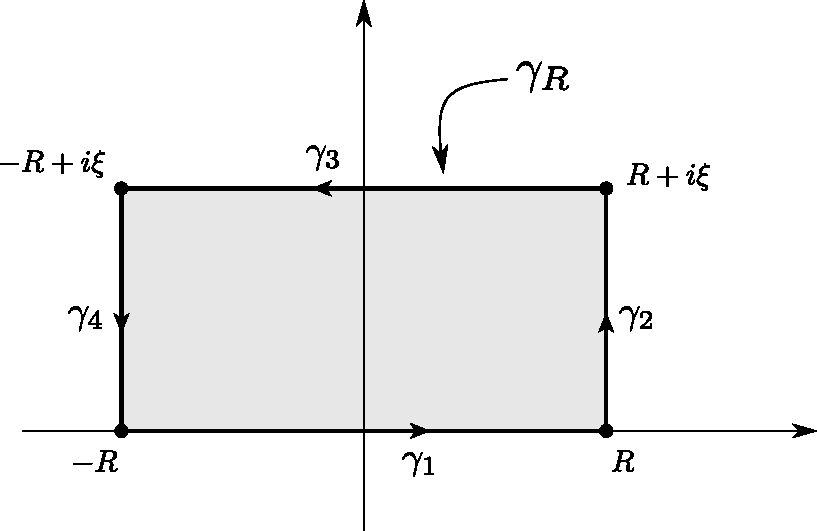
\includegraphics[width=0.6\linewidth]{Figuras/caminho-gamaR-transf-Fourier-gaussiana.pdf}
            \caption{Esboço do traço do caminho $\y_{R}$, orientado positivamente.}
            \label{fig:cont-transf-fourier-gaussiana}
        \end{figure}
        %
        Os caminhos suaves $\y_1,\y_2,\y_3$ e $\y_4$ podem ser parametrizadas da seguinte forma:
        %
        \begin{equation*}
            \begin{array}{ll}
                \y_1(t) = t,				&-R\leqslant t\leqslant R;
                \\[0.15cm]
                \y_2(t) = R+it,				&\phantom{-}0\leqslant t\leqslant \xi;
                \\[0.15cm]
                \y_3^{-}(t) = t+i\xi,		&-R\leqslant t\leqslant R;
                \\[0.15cm]
                \y_4^{-}(t) = -R+it,		&\phantom{-}0\leqslant t\leqslant \xi.
            \end{array}
        \end{equation*}
        %
        Ademais, note que a função $g:\C\to\C$ dada por 
        $g(z)=e^{-\pi z^2}$ é uma função inteira. Como, para cada $R>0$, 
        o caminho $\y_R$ é um caminho fechado suave por partes, 
        então temos do Teorema de Cauchy-Goursat que
        %
        \begin{equation*}
            \int_{\y_R} g(z)\, dz=0.
        \end{equation*}
        %
        Vamos estimar primeiro a integral de $g$ ao longo de $\y_2$ usando o Lema Técnico:
        %
        \begin{align*}
            \left| \int_{\y_2} g(z)\, dz \right|
            &=
            \left| \int_{0}^{\xi} g(\y_2(t))\,\y_2'(t)\, dt \right|
            \\[0.3cm]
            &=
            \left| \int_{0}^{\xi} g(R+it)\,i\, dt \right|
            \\[0.3cm]
            &=
            \left| \int_{0}^{\xi} \exp(-\pi(R^2+2Rit-t^2)) \, dt \right|
            \\[0.3cm]
            &=
            \left| \int_{0}^{\xi} \exp(-\pi R^2) \exp(-2\pi iRt) \exp(\pi t^2) \, dt \right|
            \\[0.3cm]
            &\leqslant
            \int_{0}^{\xi} \exp(-\pi R^2) |\exp(-2\pi iRt)| \exp(\pi t^2) \, dt
            \\[0.3cm]
            &\leqslant
            \int_{0}^{\xi} \exp(-\pi R^2)\, dt
            \\[0.3cm]
            &=
            \xi \exp(-\pi R^2).
        \end{align*}
        %
        De maneira completamente análoga podemos estimar a integral de $g$ ao longo de $\y_4$.
        Do exposto acima, temos que
        %
        \begin{align*}
            0 
            &= \int_{\y_{R}} g(z)\, dz 
            \\
            &=
            \int_{\y_1} g(z)\, dz+\int_{\y_2} g(z)\, dz+\int_{\y_3} g(z)\, dz+\int_{\y_4} g(z)\, dz.
        \end{align*}
        %
        Portanto, segue que 
        %
        \begin{equation*}
            \int_{\y^{-}_3} g(z)\, dz = \int_{\y_1} g(z)\, dz + 
            \int_{\y_2} g(z)\, dz+\int_{\y_4} g(z)\, dz.
        \end{equation*}
        %
        Logo, pela definição de integral complexa e da igualdade acima, temos
        %
        \begin{align*}
            \int_{-R}^{R} e^{-\pi(t+i\xi)^2}\, dt
            &=
            \int_{\y^{-}_3} g(z)\, dz 
            \\[0.3cm]
            &=
            \int_{\y_1} g(z)\, dz + 
            \int_{\y_2} g(z)\, dz+\int_{\y_4} g(z)\, dz
            \\[0.3cm]
            &=
            \int_{-R}^{R} g(\y(t))\y'_{1}(t)\, dt + 
            \int_{\y_2} g(z)\, dz+\int_{\y_4} g(z)\, dz
            \\[0.3cm]
            &=
            \int_{-R}^{R} e^{-\pi t^2}\, dt + 
            \int_{\y_2} g(z)\, dz+\int_{\y_4} g(z)\, dz.
        \end{align*}
        %
        Podemos agora tomar o limite quando $R\to\infty$ em ambos
        lados da igualdade acima em seguida usar a identidade
        %
        \begin{equation*}
            \lim_{R\to\infty} \int_{-R}^R e^{-\pi x^2} \, dx = 1,
        \end{equation*}
        %
        para obter
        %
        \begin{equation*}
            \int_{-\infty}^{\infty} e^{-\pi(t+i\xi)^2}\, dt
            =
            \int_{-\infty}^{\infty} e^{-\pi t^2}\, dt = 1.
        \end{equation*}
        %
        Desenvolvendo o quadrado no integrando da integral que aparece
        à esquerda na igualdade acima, ficamos com
        %
        \begin{equation*}
            \int_{-\infty}^{\infty} e^{-\pi t^2} e^{-2\pi i t\xi }  e^{\pi\xi^2}\, dt = 1
            \quad \Longrightarrow\quad 
            \int_{-\infty}^{\infty} e^{-\pi t^2} e^{2\pi i t\xi } \, dt = e^{-\pi\xi^2},
        \end{equation*}
        %
        o que mostra que a transformada de Fourier de $f$ é ela mesma, como afirmado.
        Um último comentário é adequado: mostrar que a transformada de Fourier da
        gaussiana é ela mesma aponta para a {\bf possibilidade} de que a transformada
        de Fourier tenha inversa, uma vez que ela admite ``ponto fixo''. Veremos que,
        sob certas condições, essa inversa realmente existe. Uma discussão interessante
        acerca das funções cujas transformadas de Fourier são elas próprias pode ser
        encontrada \href{https://math.stackexchange.com/questions/728670/functions-that-are-their-own-fourier-transform}{neste link}.
        %
    \subsection{Existência da transformada de Fourier em \texorpdfstring{$\mathfrak{F}_a$}{Fa}}
        %
        Nesta subseção, vamos mostrar que a transformada de Fourier está bem definida em cada $\mathfrak{F}_a$.
        Para tanto, considere a sequência $(a_n)_{n\in\N}$ de números complexos dados por
        %
        \begin{equation*}
            a_n = \int_{-n}^n f(\xi + ib)e^{2\pi ik\xi} \, d\xi, \forall n\in\N,
        \end{equation*}
        %
        sendo $k\in\Z$ e $0<b<a$ fixados. Afirmamos que
        %
        \begin{proposicao}
        \label{prop-transf-fourier-definida-fa}
            Existe $I \equiv I(k,b) \in\C$ tal que $a_n\xrightarrow{n\to\infty} I$.
        \end{proposicao}
        %
        \begin{proof}
            Para mostrar o enunciado, vamos mostrar que $(a_n)_{n\in\N}$ é de Cauchy.
            
            Lembrando que $f\in\mathfrak{F}_a$, dado $\e>0$ podemos encontrar $n_0\in\N$ 
            tal que se $n \geq n_0$ então
            %
            \begin{align*}
                \left| \int_{\R\setminus[-n,n]} f(\xi + ib)e^{2\pi ik\xi} \, d\xi \right| 
                &\leq \int_{\R\setminus[-n,n]} |f(\xi + ib)| \, d\xi \\
                &\leq \int_{\R\setminus[-n,n]} \frac{A}{1+\xi^2} \, d\xi \\
                &< \e,
            \end{align*}
            %
            onde
            %
            \begin{equation*}
                \int_{\R\setminus[-n,n]} = \int_{-\infty}^{-n} + \int_n^{+\infty}.
            \end{equation*}
            %
            Assim, tomando $m,n\geq n_0$ (e supondo s.p.g. que $m>n$), temos
            %
            \begin{align*}
                |a_m - a_n| &= \left| \int_{-m}^m f(\xi + ib)e^{2\pi ik\xi} \, d\xi 
                            - \int_{-n}^n f(\xi + ib)e^{2\pi ik\xi} \, d\xi \right| \\
                            &= \left| \int_{-m}^{-n} f(\xi + ib)e^{2\pi ik\xi} \, d\xi 
                            + \int_{n}^m f(\xi + ib)e^{2\pi ik\xi} \, d\xi \right| \\
                            &\leq \int_{-m}^{-n} |f(\xi + ib)| \, d\xi 
                            + \int_{n}^m |f(\xi + ib)| \, d\xi \\
                            &\leq \int_{\R\setminus[-n,n]} |f(\xi + ib)| \, d\xi \\
                            &\leq \int_{\R\setminus[-n,n]} \frac{A}{1+\xi^2} \, d\xi \\
                            &< \e.
            \end{align*}
            %
            Portanto, $(a_n)_{n\in\N}$ é de Cauchy e, da completude de $\C$, segue a afirmação.
        \end{proof}
        %
        \begin{corolario}
            Para quaisquer $k\in\Z$ e $0\leq b < a$ fixados existe o limite
            %
            \begin{equation*}
                \lim_{N\to +\infty} \int_{-N}^N f(\xi + ib) e^{\pm 2\pi ik\xi} 
                \equiv \int_{-\infty}^{\infty} f(\xi + ib) e^{\pm 2\pi ik\xi}.
            \end{equation*}
            %
        \end{corolario}
        %
        \begin{proof}
            Dado $\e>0$, tome $I\equiv I(k,b)$ dado na proposição anterior e seja $n = \lfloor N \rfloor$. 
            Então existe $n_0\in\N$ tal que $N\geq n_0$ implica que
            %
            \begin{align*}
                \left| \int_{-N}^N f(\xi + ib)e^{2\pi ik\xi} \, d\xi - I \right| 
                &\leq \left| \int_{-N}^N f(\xi + ib)e^{2\pi ik\xi} \, d\xi 
                - \int_{-n}^n f(\xi + ib)e^{2\pi ik\xi} \, d\xi \right| \\
                &+ \left| \int_{-n}^n f(\xi + ib)e^{2\pi ik\xi} \, d\xi - I \right| \\
                &< \int_{\R\setminus[-n,n]} |f(\xi + ib)| \, d\xi + \frac{\e}{2} \\
                &< \e.
            \end{align*}
            %
            Esse resultado nos diz, essencialmente, que os limites $n$ e $-n$ da integração podem
            ser tomados como números reais e não apenas inteiros. A rigor, é esse o resultado que mostra
            que a transformada de Fourier está bem definida em cada $\mathfrak{F}_a$.
        \end{proof}
        %
    \subsection{Ação da transformada de Fourier em \texorpdfstring{$\mathfrak{F}$}{F}}
        %
        \begin{teorema}
        \label{teo-transf-fourier-decai-exp}
            Se $f\in\mathfrak{F}_a$ para algum $a>0$, então
            %
            \begin{equation*}
                |\widehat{f}(\xi)| \leq Be^{-2\pi b|\xi|}, \forall 0\leq b < a.
            \end{equation*}
            %
        \end{teorema}
        %
        \begin{proof}
            Recorde que
            %
            \begin{equation*}
            \widehat{f}(\xi) = \int_{-\infty}^{\infty} f(x) e^{-2\pi ix\xi} \, dx.
            \end{equation*}
            %
            Se $b=0$, então
            %
            \begin{align*}
                |\widehat{f}(\xi)| &= \left| \int_{-\infty}^{\infty} f(x) e^{-2\pi ix\xi} \, dx \right| \\
                                   &\leq \int_{-\infty}^{\infty} |f(x)|\cdot |e^{-2\pi ix\xi}| \, dx \\
                                   &\leq \int_{-\infty}^{\infty} \frac{A}{1+x^2} \, dx \\
                                   &= A\pi < +\infty,
            \end{align*}
            %
            o que prova a afirmação tomando-se $B=A\pi$.
            
            Agora, suponhamos que $0 < b < a$ e assumamos inicialmente que $\xi > 0$.
            A estratégia será usar a teoria de Cauchy para deformar o contorno de integração e obter
            o decaimento desejado.
            
            Considere então a função $g$ dada por $g(z) = f(z)\exp(-2\pi iz\xi)$. Observe que $\xi$
            está fixado. Consideramos então o contorno mostrado no diagrama abaixo.
            %
            \begin{figure}[H]
				\centering 
				\begin{tikzpicture}
				\draw (4,0)--(4,-3)--(-4,-3)--(-4,0)--cycle;
				\draw[-latex] (-5,0)--(5,0) node [at end,right]{$\Re$};
				\draw[-latex] (0,-4)--(0,2) node [at end,above]{$\Im$};
				\node[at={(4,0)}, above]{$R$};
				\node [at= {(4,-3)}, below]{$R-ib$};
				\node[at={(-4,-3)}, below]{$-R-ib$};
				\node [at= {(-4,0)}, above]{$-R$};
				\node [at={(2.7,0)}, above]{$\y_1$};
				\node [at={(4,-2.2)}, right]{$\y_2$};
				\node [at={(-2,-3)}, below]{$\y_3$};
				\node [at={(-4,-1.2)}, left]{$\y_4$};
				\draw[->] (2.5,0)--(2.9,0);
				\draw[->] (4,-2)--(4,-2.2);
				\draw[->] (-1.8,-3)--(-2,-3);
				\draw[->] (-4,-1.3)--(-4,-1.2);
				\end{tikzpicture}
				\caption{Contorno no caso $\xi > 0$.}
			\end{figure}
            %
            Daí, temos que
            %
            \begin{align*}
                \left|\int_{\y_4} g(z) \, dz\right| &= \left|\int_{-R-ib}^{-R} g(z) \, dz\right| \\
                                                        &\leq \int_0^b \left| f(-R-it)e^{-2\pi i(R-it)\xi}
                                                        \right|\, dt \\
                                                        &\leq \int_0^b \frac{A}{R^2}e^{-2\pi t\xi} \, dt \\
                                                        &= \frac{K}{R^2}.
            \end{align*}
            %
            Analogamente, mostra-se que
            %
            \begin{equation*}
                \left|\int_{\y_2} g(z) \, dz\right| \leq \frac{\widetilde{K}}{R^2}.
            \end{equation*}
            %
            Pelo Teorema de Cauchy, temos
            %
            \begin{align*}
                0 = \int_{\y_1*\y_2*\y_3*\y_4} g(z) \, dz 
                \implies -\int_{\y_3} g(z) \, dz = \int_{\y_1} g(z) \, dz 
                                                     + \int_{\y_2*\y_4} g(z) \, dz.
            \end{align*}
            %
            Por definição de integral complexa, temos
            %
            \begin{align*}
                -\int_{\y_3} g(z) \, dz &= \int_{\y_3^-} g(z) \, dz \\
                                            &= \int_{-R}^R g(x-ib) \, dx \\
                                            &= \int_{-R}^R f(x-ib)e^{-2\pi i(x-ib)\xi} \, dx
            \end{align*}
            %
            e também
            %
            \begin{equation*}
                \int_{\y_1} g(z) \, dz = \int_{-R}^R g(x) \, dx = \int_{-R}^R f(x)e^{-2\pi ix\xi} \, dx.
            \end{equation*}
            %
            Tomando o limite para $R\to +\infty$, obtemos
            %
            \begin{align*}
                \int_{-\infty}^{\infty} f(x-ib)e^{-2\pi i(x-ib)\xi} \, dx
                =
                \int_{-\infty}^{\infty} f(x)e^{-2\pi ix\xi} \, dx
                =
                \widehat{f}(\xi),
            \end{align*}
            %
            donde segue que
            %
            \begin{align*}
                |\widehat{f}(\xi)| &=\left|\int_{-\infty}^{\infty} f(x-ib)e^{-2\pi i(x-ib)\xi} \, dx\right| \\
                                   &\leq\int_{-\infty}^{\infty}|f(x-ib)|e^{-2\pi ix\xi}e^{-2\pi i(-ib)\xi}\,dx \\
                                   &= \int_{-\infty}^{\infty}|f(x-ib)|e^{-2\pi b\xi} \,dx \\
                                   &= \int_{-\infty}^{\infty}|f(x-ib)|e^{-2\pi b|\xi|} \,dx \\
                                   &\leq \int_{-\infty}^{\infty} \frac{A}{1+x^2}e^{-2\pi b|\xi|} \, dx \\
                                   &= Be^{-2\pi b|\xi|}.
            \end{align*}
            %
            Isso prova o resultado para $\xi > 0$. Para $\xi < 0$, procedemos de maneira análoga considerando
            o contorno abaixo.
            %
            \begin{figure}[H]
				\centering 
				\begin{tikzpicture}
				\draw (4,0)--(4,3)--(-4,3)--(-4,0)--cycle;
				\draw[-latex] (-5,0)--(5,0) node [at end,right]{$\Re$};
				\draw[-latex] (0,-2)--(0,4) node [at end,above]{$\Im$};
				\node[at={(4,0)}, below]{$R$};
				\node [at= {(4,3)}, above]{$R+ib$};
				\node[at={(-4,3)}, above]{$-R+ib$};
				\node [at= {(-4,0)}, below]{$-R$};
				%\node [at={(4,1.5)}, right]{$\y_R$};
				\draw[->] (-2.3,3)--(-2.5,3);
				\draw[->] (-4,1.7)--(-4,1.5);
				\draw[->] (2.5,0)--(2.7,0);
				\draw[->] (4,2.2)--(4,2.5);
				\end{tikzpicture}
				\caption{Contorno no caso $\xi < 0$.}
			\end{figure}
            %
            Note que quanto ``mais larga'' for a faixa $S_a$ na qual podemos estender $f$, ``maior'' será o 
            decaimento de $\widehat{h}$, i.e., mais rápido ela decairá, porque poderemos escolher valores de
            $b$ maiores.
        \end{proof}
        %
        \begin{corolario}
        \label{transf-fourier-inv-por-shift}
            A demonstração do Teorema \ref{teo-transf-fourier-decai-exp} nos deu o seguinte fato,
            para todo $0\leq b < a$, sendo $a > 0$ tal que $f\in\mathfrak{F}_a$:
            %
            \begin{align*}
                \int_{-\infty}^{\infty} f(x-ib)e^{-2\pi i(x-ib)\xi} \, dx
                =
                \int_{-\infty}^{\infty} f(x)e^{-2\pi ix\xi} \, dx
                =
                \widehat{f}(\xi)
            \end{align*}
            %
            para $\xi > 0$ e
            %
            \begin{align*}
                \int_{-\infty}^{\infty} f(x+ib)e^{-2\pi i(x+ib)\xi} \, dx
                =
                \int_{-\infty}^{\infty} f(x)e^{-2\pi ix\xi} \, dx
                =
                \widehat{f}(\xi)
            \end{align*}
            %
            para $\xi < 0$.
        \end{corolario}
        %
        Separamos o fato acima como corolário pois ele será bastante usado e não é algo exclusivo da
        demonstração do Teorema \ref{teo-transf-fourier-decai-exp}. Podemos, agora, definir a classe
        $\mathfrak{F}$.
        %
        \begin{definicao}[Classe $\mathfrak{F}$]
        \label{def-classe-F}
            A classe $\mathfrak{F}$ é o espaço de todas as funções que pertencem a $\mathfrak{F}_a$
            para algum $a>0$, isto é,
            %
            \begin{equation*}
                \mathfrak{F} = \bigcup_{a>0} \mathfrak{F}_a.
            \end{equation*}
            %
        \end{definicao}
        %
        Com essa classe, podemos mostrar a validade da fórmula de inversão da transformada.
        %
        \begin{teorema}
        \label{teo-inv-transf-fourier}
            Se $f\in\mathfrak{F}$, vale a igualdade
            %
            \begin{equation*}
                f(x) = \int_{-\infty}^{\infty} \widehat{f}(\xi) e^{2\pi ix\xi} \, d\xi, \forall x\in\R.
            \end{equation*}
            %
        \end{teorema}
        %
        Para provar o lema, vamos precisar do seguinte lema.
        %
        \begin{lema}
        \label{lema-int-exp}
            Se $A>0$ e $B\in\R$, então
            %
            \begin{equation*}
                \int_0^{\infty} e^{-(A+iB)\xi} \, d\xi = \frac{1}{A+iB}.
            \end{equation*}
            %
        \end{lema}
        %
        \begin{proof}
            Esse resultado pode ser visto como um caso especial da transformada de Laplace,
            %
            \begin{equation*}
                \mathcal{L}\{f\}(s) = \int_0^{\infty} f(\xi) e^{-s\xi} \, d\xi,
            \end{equation*}
            %
            bastando tomar $f(\xi)\equiv 1$ e $s = (A+iB)$.
            
            Uma outra maneira de provar isto é ``no braço'': já que $A > 0$, temos $|e^{-(A+iB)\xi}| = e^{-A\xi}$
            e, portanto, a integral do enunciado converge. Por definição,
            %
            \begin{equation*}
                \int_0^{\infty} e^{-(A+iB)\xi} \, d\xi = \lim_{R\to\infty} \int_0^R e^{-(A+iB)\xi} \, d\xi.
            \end{equation*}
            %
            Note que
            %
            \begin{equation*}
                \int_0^R e^{-(A+iB)\xi} \, d\xi = -\frac{e^{-(A+iB)\xi}}{A+iB}\Bigg|_0^R,
            \end{equation*}
            %
            de modo que
            %
            \begin{equation*}
                \lim_{R\to\infty} \int_0^R e^{-(A+iB)\xi} \, d\xi = \frac{1}{A+iB}.
            \end{equation*}
            %
        \end{proof}
        %
        
        \begin{proof}[Prova do Teorema \ref{teo-inv-transf-fourier}]
            Aqui, novamente, precisamos estar atentos ao sinal de $\xi$. Primeiro, note que
            %
            \begin{equation*}
                \int_{-\infty}^{\infty} \widehat{f}(\xi) e^{2\pi ix\xi} \, d\xi 
                = \int_{-\infty}^{0} \widehat{f}(\xi) e^{2\pi ix\xi} \, d\xi 
                + \int_{0}^{\infty} \widehat{f}(\xi) e^{2\pi ix\xi} \, d\xi.
            \end{equation*}
            %
            Vamos começar analisando a segunda parcela.
            
            Digamos que $f\in\mathfrak{F}_a$ para algum $a>0$. Escolha $b\in\R$ tal que $0 < b < a$.
            Lembrando do Corolário \ref{transf-fourier-inv-por-shift} e usando o Teorema de Fubini, temos
            %
            \begin{align*}
                \int_{0}^{\infty} \widehat{f}(\xi) e^{2\pi ix\xi} \, d\xi
                &= \int_{0}^{\infty} \left[ \int_{-\infty}^{\infty} f(u-ib)e^{-2\pi i(u-ib)\xi} \, du \right] 
                    e^{2\pi ix\xi} \, d\xi \\
                &= \int_{-\infty}^{\infty} \left[ \int_{0}^{\infty} f(u-ib)e^{-2\pi i(u-ib)\xi}e^{2\pi ix\xi} \, d\xi
                    \right] \, du \\
                &= \int_{-\infty}^{\infty} f(u-ib) \left[ \int_{0}^{\infty} e^{-2\pi i(u-ib)\xi}e^{2\pi ix\xi} \, d\xi
                    \right] \, du \\
                &= \int_{-\infty}^{\infty} f(u-ib)\cdot\frac{1}{2\pi b + 2\pi i(u-x)} \, du \\
                &= \int_{-\infty}^{\infty} \frac{f(u-ib)}{2\pi i (-ib + u - x)} \, du \\
                &= \frac{1}{2\pi i} \int_{-\infty}^{\infty} \frac{f(\y_1(u))}{\y_1(u)-x}\, \y_1'(u) \, du \\
                &\equiv \frac{1}{2\pi i}\int_{\y_1} \frac{f(w)}{w-x} \, dw,
            \end{align*}
            %
            sendo $\y_1(u) = u-ib, u\in\R$. Procedendo de maneira análoga para a primeira parcela, obtemos
            %
            \begin{equation*}
                \int_{-\infty}^0 \widehat{f}(\xi) e^{2\pi ix\xi} \, d\xi 
                = -\frac{1}{2\pi i}\int_{\y_2} \frac{f(w)}{w-x} \, dw,
            \end{equation*}
            %
            sendo $\y_2(u) = u+ib, b\in\R$. Ilustramos os ``caminhos'' abaixo.
            %
            \begin{figure}[H]
				\centering 
				\begin{tikzpicture}
				\draw (-5,2)--(5,2);
				\draw (-5,-2)--(5,-2);
				\draw[-latex] (-5,0)--(5,0) node [at end,right]{$\Re$};
				\draw[-latex] (0,-3)--(0,3) node [at end,above]{$\Im$};
				\node [at={(0,2)}, above right]{$ia$};
				\node [at={(0,-2)}, below right]{$-ia$};
				\draw[-latex,teal] (-5,1.2)--(5,1.2) node [at end,above]{$\y_2$};
				\node [at={(0,1.2)}, above left]{$ib$};
				\draw[-latex,teal] (-5,-1.2)--(5,-1.2) node [at end,above]{$\y_1$};
				\node [at={(0,-1.2)}, above left]{$-ib$};
				\end{tikzpicture}
			\end{figure}
        %
            A estratégia agora será truncar esses dois ``caminhos'', formando o retângulo abaixo, e mostrar que
            as integrais nos caminhos verticais vão para zero quando $R\to\infty$.
            %
            \begin{figure}[H]
				\centering 
				\begin{tikzpicture}
				\draw (4,2)--(-4,2)--(-4,-2)--(4,-2)--cycle;
				\draw[-latex] (-5,0)--(5,0) node [at end,right]{$\Re$};
				\draw[-latex] (0,-4)--(0,4) node [at end,above]{$\Im$};
				\node[at={(4,0)}, below right]{$R$};
				%\node [at= {(4,-3)}, below]{$R-ib$};
				%\node[at={(-4,-3)}, below]{$-R-ib$};
				\node [at= {(-4,0)}, below left]{$-R$};
				\node [at={(2,-2)}, below]{$\beta_R^1$};
				\node [at={(4,1)}, right]{$\beta_R^2$};
				\node [at={(2,2)}, above]{$\beta_R^3$};
				\node [at={(-4,1)}, left]{$\beta_R^4$};
				\draw[-latex] (4,0.9)--(4,1);
				\draw[-latex] (4,-1.1)--(4,-1);
				\draw[-latex] (2.1,2)--(2,2);
				\draw[-latex] (-1.9,2)--(-2,2);
				\draw[-latex] (-4,1.1)--(-4,1);
				\draw[-latex] (-4,-0.9)--(-4,-1);
				\draw[-latex] (-2.1,-2)--(-2,-2);
				\draw[-latex] (1.9,-2)--(2,-2);
				\end{tikzpicture}
				\caption{Contorno no caso $\xi > 0$.}
			\end{figure}
            %
            Defina $\beta_R \equiv \beta_R^1*\beta_R^2*\beta_R^3*\beta_R^4$. Usando a Fórmula Integral de Cauchy
            e lembrando que $R > |x|$, temos
            %
            \begin{align*}
                f(x) = \frac{1}{2\pi i}\int_{\beta_R} \frac{f(w)}{w-x} \, dw
                \implies f(x) = \lim_{R\to\infty} \left( \frac{1}{2\pi i}\int_{\beta_R} \frac{f(w)}{w-x} \, dw \right).
            \end{align*}
            %
            Vamos estimar a integral ao longo de $\beta_R^4$ (e analogamente ao longo de $\beta_R^2$):
            %
            \begin{align*}
                \left| \int_{\beta_R^4} \frac{f(w)}{w-x} \, dw \right| 
                &\leq \int_{\beta_R^4} \frac{|f(w)|}{|w-x|} \, |dw| \\
                &\leq \int_{\beta_R^4} \frac{A}{1+R^2}\cdot\frac{1}{R-|x|} \, |dw| \\
                &= \frac{A}{1+R^2}\cdot\frac{1}{R-|x|}\cdot 2b \\
                &= \frac{1}{R^2}\cdot\frac{2A}{(1+1/R^2)(1-|x|/R)} \xrightarrow{R\to\infty} 0.
            \end{align*}
            %
            Como tomamos valores absolutos, a estimativa para $\beta_R^2$ é a mesma. Portanto,
            %
            \begin{align*}
                f(x) &= \lim_{R\to\infty} \left( \frac{1}{2\pi i}\int_{\beta_R} \frac{f(w)}{w-x} \, dw \right) \\
                     &= \frac{1}{2\pi i} \lim_{R\to\infty} \left( \int_{\beta_R^1} \frac{f(w)}{w-x} \, dw 
                        + \int_{\beta_R^3} \frac{f(w)}{w-x} \, dw \right) \\
                     &= \frac{1}{2\pi i}\left( \int_{\y_1} \frac{f(w)}{w-x} \, dw 
                        + \int_{\y_2^-} \frac{f(w)}{w-x} \, dw \right) \\
                     &= \int_{0}^{\infty} \widehat{f}(\xi) e^{2\pi ix\xi} \, d\xi 
                        + \int_{-\infty}^0 \widehat{f}(\xi) e^{2\pi ix\xi} \, d\xi \\
                     &= \int_{-\infty}^{\infty} \widehat{f}(\xi) e^{2\pi ix\xi} \, d\xi.
            \end{align*}
            %
        \end{proof}
        %
        
        Com essas ferramentas em mãos, podemos demonstrar a fórmula da soma de Poisson.
        %
        \begin{teorema}[Fórmula da Soma de Poisson]
        \label{teo-form-soma-poisson}
            Se $f\in\mathfrak{F}$, então
            %
            \begin{equation*}
                \sum_{n\in\Z} f(n) = \sum_{n\in\Z} \widehat{f}(n).
            \end{equation*}
            %
        \end{teorema}
        %
        Antes da demonstração, fazemos uma observação que nos será útil. Se $|w| > 1$, 
        então $|1/w| < 1$ e podemos fazer uma expansão usando a série geométrica como abaixo:
        %
        \begin{align*}
            \frac{1}{w-1} &= \frac{1}{w}\cdot\frac{1}{1-\frac{1}{w}} 
            = w^{-1}\sum_{n = 0}^{\infty}w^{-n}.
        \end{align*}
        %
        Analogamente, se $|w|<1$, temos
        %
        \begin{align*}
            \frac{1}{w-1} &= -\frac{1}{1-w}
            = -\sum_{n = 0}^{\infty}w^{n}.
        \end{align*}
        %
        \begin{proof}
            Como $f\in\mathfrak{F}$, existe $a > 0$ tal que $f\in\mathfrak{F}_a$. Seja 
            $b$ um número real que satisfaz $0<b<a$. A função $1/(e^{2\pi i z} - 1)$ 
            tem polos simples sobre os números inteiros, então
            %
            \begin{equation*}
                g(z) = \frac{f(z)}{e^{2\pi i z} - 1}
            \end{equation*}
            %
            tem os mesmos polos simples, já que $f$ é holomorfa em $S_a$. 
            
            Observe ainda que, com $n \in \Z$,
            %
            \begin{align*}
                \lim_{z \to n} (z-n)g(z) & = \lim_{z \to n} \frac{(z-n)f(z)}{e^{2\pi i z} - 1}\\
                &= \lim_{z \to n} \frac{f(z) + (z-n)f'(z)}{2\pi ie^{2\pi i z}} \\
                &= \frac{f(n)}{2\pi i},
            \end{align*}
            %
            ou seja, o resíduo de $g$ em $n \in \Z$ é $f(n)/2\pi i$. Para o cálculo do limite acima,
            usamos a regra de L'Hôpital.
            
            Considere o contorno $\y_N$ na figura abaixo. 
            %
            \begin{center}
                {\bf diagrama slide 6 aula 10}
            \end{center}
            %
            Pelo teorema dos resíduos, temos que 
            %
            \begin{align*}
                \int_{\y_N}g(z)\,dz &= 2\pi i\sum_{n=-N}^{N}\res(g,n)\\
                &= 2 \pi i\sum_{n=-N}^{N}\frac{f(n)}{2 \pi i}\\
                &= \sum_{n=-N}^{N}f(n).
            \end{align*}
            %
            O resultado que procuramos será obtido quando tomarmos o limite $N \to \infty$. 
            
            Separe o contorno $\y_N$ em quatro curvas conforme o diagrama abaixo. 
            %
            \begin{center}
                {\bf slide 11 Aula 11}
            \end{center}
            %
            As integrais sobre
            $\y_N^e$ e $\y_N^d$ vão a zero quando $N \to \infty$. Para verificar isto, usamos o 
            Lema Técnico (Lema \ref{lema-tecnico}) e a hipótese de decaimento quadrático sobre $f$. 
            Denotaremos $R = N + 1/2$.
            %
            \begin{align*}
                \left |\int_{\y_N^d} \frac{f(z)}{e^{2 \pi i z} - 1}\,dz\right| 
                &\leq \int_{\y_N^d} \frac{|f(z)|}{|e^{2 \pi i z} - 1|}\,|dz| \\
                &\leq \int_{\y_N^d} \frac{A}{1 + R^2}\cdot\frac{1}{|e^{2 \pi i z} - 1|}\,|dz| \\
                &\leq \int_{\y_N^d} \frac{A}{1 + R^2}\cdot\frac{1}{e^{-2\pi b} + 1}\,|dz| \\
                & = \frac{A2b}{(1 + R^2)(e^{-2\pi b} + 1)} \xrightarrow{N \to \infty} 0.
            \end{align*}
            %
            Na terceira desigualdade, usamos o fato que $|e^{2\pi i z} - 1| \geq e^{-2 \pi b} + 1$ 
            para $z \in \y_N^d$. Para $t \in [-b,b]$,
            %
            \begin{align*}
                |e^{2 \pi i z} - 1| &= |e^{2 \pi i(R+ + i t)} - 1| \\
                &= |e^{\pi i}e^{-2\pi t} - 1| \\
                & = |(-1)e^{-2\pi t} - 1| \\
                &= |e^{-2\pi t} + 1| \\
                &\geq e^{-2\pi b} + 1.
            \end{align*}
            %
            Vamos denotar por $\y^1$ e $\y^2$ as partes inferior e superior, respectivamente, 
            do contorno $\y_N$ quando $N \to \infty$. Pelo que vimos até aqui,
            %
            \begin{equation*}
                \sum_{n \in \Z}f(n) = \int_{\y^1}\frac{f(z)}{e^{2\pi i z} - 1}\,dz 
                                    + \int_{\y^2}\frac{f(z)}{e^{2\pi i z} - 1}\,dz.
            \end{equation*}
            %
            A parametrização de $\y^1$ é $t - ib$ com $t \in \R$, então, para $z \in \y^1$, 
            temos 
            %
            \begin{equation*}
                |e^{2\pi i z}| = |e^{2\pi i(t - ib)}| = |e^{2\pi it}e^{2\pi b}| = e^{2\pi b} >1.
            \end{equation*}
            %
            Pela observação que fizemos antes da demonstração,
            %
            \begin{equation*}
             \frac{1}{e^{2\pi i z}-1} = e^{-2\pi i z}\sum_{n=0}^{\infty}e^{-2\pi i nz}.
            \end{equation*}
            %
            Para $z \in \y^2$, temos
            %
            \begin{equation*}
                |e^{2\pi i z}| = |e^{2\pi i(-t + ib)}| = |e^{-2\pi it}e^{-2\pi b}| = e^{-2\pi b} <1
            \end{equation*}
            %
            e segue
            %
            \begin{equation*}
                \frac{1}{e^{2\pi i z}-1} = -\sum_{n=0}^{\infty}e^{2\pi i nz}.
            \end{equation*}
            %
            Portanto
            %
            \begin{align*}
                \sum_{n \in \Z}f(n) &= \int_{\y^1} f(z) e^{-2\pi i z} 
                \sum_{n=0}^{\infty} e^{-2\pi i nz}\,dz 
                + \int_{\y^2} f(z)(-1) \sum_{n=0}^{\infty} e^{2\pi i nz}\,dz\\
                &= \int_{-\infty}^{\infty}f(\xi - ib)e^{-2\pi i (\xi - ib)}
                \sum_{n=0}^{\infty}e^{-2\pi i n(\xi - ib)}\,d\xi 
                + \int_{-\infty}^{\infty}f(\xi - ib)
                \sum_{n=0}^{\infty}e^{2\pi i n(\xi - ib)}\,d\xi \\
                &= \sum_{n=0}^{\infty} \int_{-\infty}^{\infty}f(\xi - ib)
                e^{-2\pi i (n+1)(\xi - ib)}\,d\xi 
                + \sum_{n=0}^{\infty} \int_{-\infty}^{\infty}f(\xi - ib)(-1)
                e^{2\pi i n(\xi - ib)}\,d\xi \\
                &= \sum_{n=0}^{\infty} \hat{f}(n+1) + \sum_{n=0}^{\infty} \hat{f}(-n) \\
                &= \sum_{n \in \Z} \hat{f}(n).
            \end{align*}
            %
        \end{proof}
        %
        
        Observe que no final da demonstração anterior usamos que, no cálculo da 
        transformada de Fourier, podemos mudar a reta por onde integramos, como mostrado 
        na demonstração do Teorema \ref{teo-transf-fourier-decai-exp}. Além disso, trocamos
        a ordem da série com o somatório sem dar muitas justificativas. 
        O que justifica essa troca é o lema a seguir.
        %
        \begin{lema}
            Seja $f \in \mathfrak{F}_a$. Para qualquer $b$ real satisfazendo $0 < b < a$, 
            temos que os seguintes limites
            %
            \begin{equation*}
            \int_{-\infty}^{\infty}f(\xi + ib)\sum_{n=0}^{\infty}e^{2\pi i n(\xi + ib)}\,d\xi, 
            \hspace{7pt}
            \sum_{n=0}^{\infty} \int_{-\infty}^{\infty}f(\xi + ib)e^{2\pi ni(\xi + ib)}\,d\xi
            \end{equation*}
            %
            existem e são iguais.
        \end{lema}
        %
        \begin{proof}
            Vamos denotar por $I$ e por $II$ os limites à esquerda e à direita, respectivamente, 
            no enunciado. Começamos observando que cada parcela em $II$ é bem definida, e vamos mostrar 
            que essa série converge absolutamente:
            %
            \begin{align*}
                \sum_{n=0}^{\infty}\left|\int_{-\infty}^{\infty} f(\xi + ib)
                e^{2 \pi i n(\xi + i b)} \, d\xi\right| 
                &\leq \sum_{n=0}^{\infty}\int_{-\infty}^{\infty} |f(\xi + ib)|
                e^{-2 \pi nb} \, d\xi \\
                &\leq \sum_{n=0}^{\infty}e^{-2 \pi nb}\int_{-\infty}^{\infty} \frac{A}{1 + \xi^2}\, d\xi \\
                &= A\pi\sum_{n=0}^{\infty}e^{-2 \pi nb}
                < \infty,
            \end{align*}
            %
        onde usamos que a série geométrica
        %
        \begin{equation*}
            \sum_{n=0}^{\infty}e^{-2 \pi nb}
        \end{equation*}
        %
        converge pois $b > 0$.
        
        Para ver que $I$ converge, lembre-se que
        %
        \begin{equation*}
            \sum_{n=0}^{\infty} e^{2\pi n i(\xi + ib)} = \frac{1}{1 - e^{2\pi i(\xi + ib)}},
        \end{equation*}
        %
        uma vez que
        %
        \begin{equation*}
            |e^{2\pi n i(\xi + ib)}| = e^{-2\pi nb} < 1
        \end{equation*}
        %
        para $b,n > 0$. Assim, $I$ se escreve como
        %
        \begin{equation*}
            \int_{-\infty}^{\infty} f(\xi + ib)\frac{1}{1 - e^{2\pi i(\xi + ib)}}\,d\xi.
        \end{equation*}
        %
        Temos que $\exp(2\pi i (\xi + ib)) = \exp(-2\pi b + i2\pi \xi)$ e, 
        conforme $\xi$ varia, esse número percorre uma circunferência de raio 
        $e^{-2\pi b} < 1$ com centro na origem. Portanto, 
        $|1 - e^{2\pi i(\xi + ib)}| \geq 1 - e^{-2\pi b}$, como mostrado no 
        diagrama abaixo.
        %
        \begin{center}
            {\bf diagrama do descrito acima}
        \end{center}
        %
        Logo,
        %
        \begin{align*}
            |I| &\leq \int_{-\infty}^{\infty}|f(\xi + ib)|\frac{1}{|1 - e^{2\pi i(\xi + ib)}|} \, d\xi \\
            &\leq \frac{1}{1 - e^{-2\pi b}}\int_{-\infty}^{\infty} \frac{A}{1 + \xi^2} \, d\xi < \infty.
        \end{align*}
        %
        Defina, para cada $N\in \N$,
        %
        \begin{equation*}
            I_N = \int_{-N}^{N}f(\xi + ib)\frac{1}{1 - e^{2\pi i(\xi + ib)}} \, d\xi,
        \end{equation*}
        %
        que é finita para cada $N$ (basta estimar $I_N$ como estimamos $I$).
        Por definição, $I = \displaystyle{\lim_{N\to\infty} I_N}$. 
        Finalmente, vamos mostrar que $I = II$ 
        analisando o módulo da diferença entre eles.
        %
        \begin{equation*}
            |I - II|  = |I - I_N + I_N - II| \leq |I-I_N| + |I_N - II|.
        \end{equation*}
        %
        Como $|I - I_N| \to 0$ conforme $N \to \infty$, basta mostrar que, também, 
        $|I_N - II| \to 0$. Vamos denotar por $F(\xi,b)$ a expressão 
        $f(\xi + ib)/(1 - e^{2\pi i(\xi + ib)})$ e por $F_n(\xi,b)$ a expressão 
        $f(\xi + ib)e^{2\pi in(\xi + ib)}$. Desse modo, temos
        %
        \begin{align*}
            I_N - II &= \int_{-N}^{N} \frac{f(\xi + ib)}{(1 - e^{2\pi i(\xi + ib)})}
            \, d\xi - \sum_{n=0}^{\infty}\int_{-\infty}^{\infty} f(\xi + ib)
            e^{2\pi in(\xi + ib)} \, d\xi \\
            %
            &=\int_{-N}^{N} F(\xi,b) \, d\xi -
            \sum_{n=0}^{\infty}\int_{-\infty}^{\infty}F_n(\xi,b) \, d\xi \\
            %
            &= \int_{-N}^{N} F(\xi,b) \, d\xi - 
            \sum_{n=0}^{N}\int_{-\infty}^{\infty}F_n(\xi,b) \, d\xi - 
            \sum_{n= N+1}^{\infty}\int_{-\infty}^{\infty}F_n(\xi,b) \, d\xi\\
            %
            &= \int_{-N}^{N} F(\xi,b) \, d\xi - \int_{-\infty}^{\infty} 
            \sum_{n=0}^{N}F_n(\xi,b) \, d\xi - 
            \sum_{n= N+1}^{\infty}\int_{-\infty}^{\infty}F_n(\xi,b) \, d\xi\\
            %
            &= \underbrace{\int_{-N}^{N} \left(F(\xi,b) - \sum_{n=0}^{N}F_n(\xi,b) 
            \right)\, d\xi}_{(*)} - 
            \underbrace{\int_{\R \setminus [-N,N]}\sum_{n=0}^{N}F_n(\xi,b) 
            \, d\xi}_{(**)} \\ &- 
            \underbrace{\sum_{n= N+1}^{\infty}\int_{-\infty}^{\infty}F_n(\xi,b) 
            \, d\xi.}_{(***)}
        \end{align*}
        %
        Vamos estimar cada parte separadamente. Para $(*)$, temos
        %
        \begin{align*}
            &\left|\int_{-N}^{N} f(\xi + ib)\left(\frac{1}{1 - e^{2\pi i(\xi + ib)}} - \sum_{n=0}^{N}e^{2\pi i n(\xi + ib)}\right) \, d\xi \right| \\
            %
            &\leq \int_{-N}^{N} |f(\xi + ib)|\cdot\left|\frac{1}{1 - e^{2\pi i(\xi + ib)}} - \sum_{n=0}^{N}e^{2\pi i n(\xi + ib)}\right| \, d\xi \\
            %
            &\leq \int_{-N}^{N} \frac{A}{1 + \xi^2}\left|\frac{1}{1 - e^{2\pi i(\xi + ib)}} - \sum_{n=0}^{N}e^{2\pi i n(\xi + ib)}\right| \, d\xi 
        \end{align*}
        %
        Por conta da série geométrica, sabemos que, dado $\e>0$, existe 
        $N$ suficientemente grande tal que
        %
        \begin{equation*}
            \left|\frac{1}{1 - e^{2\pi i(\xi + ib)}} - 
            \sum_{n=0}^{N}e^{2\pi i n(\xi + ib}\right| < \e. 
        \end{equation*}
        %
        Concluímos então que a parte em $(*)$ vai a $0$ quando $N \to \infty$. 
        %
        A parte em $(***)$ é a cauda da série que definimos como $II$, 
        que é convergente, então a expressão em $(***)$ deve ir a $0$. 
        Por fim, a expressão em $(**)$ se parece com a cauda da integral $I$.
        Estimando-a, temos
        %
        \begin{align*}
            \left|\int_{\R \setminus [-N,N]}\sum_{n=0}^{N}F_n(\xi,b) \, d\xi\right| 
            %
            &= \left|\int_{\R \setminus [-N,N]}f(\xi + ib)\sum_{n=0}^{N}
            e^{2\pi i n(\xi + ib)} \, d\xi\right| \\
            %
            &\leq \int_{\R \setminus [-N,N]}|f(\xi + ib)|\left|\sum_{n=0}^{N}
            e^{2\pi i n(\xi + ib)} \right|\, d\xi \\
            %
            &\leq \int_{\R \setminus [-N,N]}\frac{A}{1 + \xi^2} 
            \sum_{n=0}^{N}|e^{2\pi i n(\xi + ib)}| \, d\xi \\
            %
            &\leq \int_{\R \setminus [-N,N]}\frac{A}{1 + \xi^2}
            \sum_{n=0}^{\infty}e^{-2\pi i nb} \, d\xi. 
        \end{align*}
        %
        Como 
        %
        \begin{equation*}
            \sum_{n=0}^{\infty}e^{-2\pi i nb}
        \end{equation*}
        %
        é finito, concluímos que 
        a última expressão vai a zero quando $N \to \infty$. Com isso, 
        $(*), (**)$ e $(***)$ vão a zero, então temos que $|I - II|< \e$ para 
        qualquer $\e>0$ dado, ou seja, $I = II$.
        \end{proof}
        %
    \subsection{O teorema de Paley-Wiener}
        Nesta seção vamos adotar um ponto de vista um pouco diferente acerca da nossa $f:\R\to\R$: 
        ao invés de assumir qualquer analiticidade em $f$, vamos assumir a validade da fórmula de 
        inversão de Fourier, isto é,
        que vale
        %
        \begin{equation*}
            f(x) = \int_{-\infty}^{\infty} \widehat{f}(\xi) e^{2\pi ix\xi} \, d\xi
        \end{equation*}
        %
        se
        %
        \begin{equation*}
            \widehat{f}(x) = \int_{-\infty}^{\infty} f(x) e^{-2\pi ix\xi} \, dx.
        \end{equation*}
        %
        Dito de outro modo, vamos trabalhar com funções para as quais existe a transformada de Fourier
        e vale a fórmula de inversão dada no Teorema \ref{teo-inv-transf-fourier}. A esta segunda
        hipótese, chamaremos {\bf Hipótese da Fourier Inversa}, H.F.I.
        
        É possível mostrar, ainda, que a existência da transformada de Fourier e o 
        Teorema \ref{teo-inv-transf-fourier} podem ser obtidos fazendo-se as seguintes hipóteses
        sobre $f$ e $\widehat{f}$:
        %
        \begin{align*}
            \forall x\in\R, |f(x)| &\leq \frac{A}{1+x^2}; \\
            \forall \xi\in\R, |\widehat{f}(\xi)| &\leq \frac{A'}{1+\xi^2},
        \end{align*}
        %
        com $A,A' > 0$ constantes.
        %
        \begin{teorema}
        \label{teo-extensao-analitica-transf-decai-exp}
            Seja $f:\R\to\R$ uma função satisfazendo H.F.I. e tal que para algumas constantes $a,A > 0$
            temos $|\widehat{f}(\xi)| \leq Ae^{-2\pi a|\xi|}$. Então, para todo $b\in\R$ tal que 
            $0<b<a$, $f$ admite uma extensão analítica à faixa $S_b = \{ z\in\C \ : \ |\Im(z)| < b \}$,
            ou seja, existe uma função $F:S_b\to\C$ holomorfa tal que $F\big|_{\R} \equiv f$.
        \end{teorema}
        %
        \begin{proof}
            Defina
            %
            \begin{equation*}
                f_n(z) = \int_{-n}^{n} \widehat{f}(\xi) e^{2\pi iz\xi} \, d\xi.
            \end{equation*}
            %
            A rigor, para o que faremos a seguir, seria necessário mostrar que $f_n(z)$ está bem
            definida (no contexto da integração de Riemann), mostrando que $\widehat{f}$ é contínua
            e o integrando é limitado para cada $z$ fixo. No contexto de teoria da medida, 
            não precisaríamos nos preocupar com isso. No que segue, vamos supor $f_n(z)$ bem 
            definida sem demonstração, mas é possível mostrar isso. Além disso, vamos
            também utilizar o teorema de Fubini para trocar a ordem de integração 
            (o que, a rigor, também precisaria ser demonstrado como permitido).
            
            Já que para qualquer curva de Jordan suave por partes em $\C$ temos
            %
            \begin{align*}
                \int_{\y} f_n(z) \, dz &= \int_{\y} \int_{-n}^n \widehat{f}(\xi) e^{2\pi iz\xi} \, d\xi \, dz \\
                                       &= \int_{-n}^n \left[ \int_{\y} \widehat{f}(\xi)e^{2\pi iz\xi} \, dz 
                                        \right] \, d\xi \\
                                       &= \int_{-n}^n \widehat{f}(\xi) \left[ \int_{\y} e^{2\pi iz\xi} \, dz
                                       \right] \, d\xi = 0,
            \end{align*}
            %
            segue do Teorema de Morera que $f_n:\C\to\C$ é uma função inteira.
            
            Ademais, uma vez que $|\widehat{f}(\xi)| \leq Ae^{-2\pi a|\xi|}$, a seguinte expressão 
            está bem definida para todo $z\in S_b$:
            %
            \begin{equation*}
                F(z) = \int_{-\infty}^{\infty} \widehat{f}(\xi) e^{2\pi iz\xi} \, d\xi.
            \end{equation*}
            %
            De fato,
            %
            \begin{align*}
                \left| \int_{\R\setminus [-n,n]} \widehat{f}(\xi) e^{2\pi iz\xi} \, d\xi \right|
                &\leq \int_{\R\setminus [-n,n]} |\widehat{f}(\xi)|e^{2\pi b|\xi|} \, d\xi \\
                &\leq \int_{\R\setminus [-n,n]} Ae^{-2\pi (a-b)|\xi|} \, d\xi \xrightarrow{n\to\infty} 0,
            \end{align*}
            %
            onde usamos que
            %
            \begin{equation*}
                \Re(2\pi iz\xi) = -2\pi\xi\Im(z) \leq 2\pi b|\xi|
            \end{equation*}
            %
            na primeira desigualdade, o decaimento de $\widehat{f}$ na segunda desigualdade e
            o fato de que $0<b<a$ para calcular o limite quando $n\to\infty$.
            
            Por fim, basta considerarmos as restrições de $f_n$ a $S_b$ e observar que a sequência
            $(f_n)_{n\in\N}$ dessas restrições converge uniformemente para $F:S_b\to\C$ dada acima.
            
            De fato, dado $\e>0$ existe $n_0\in\N$ tal que se $n\geq n_0$ então, para todo $z\in S_b$,
            %
            \begin{align*}
                |F(z) - f_n(z)| &= \left| \int_{-\infty}^{\infty} \widehat{f}(\xi) e^{2\pi iz\xi} \, d\xi -
                \int_{-n}^{n} \widehat{f}(\xi) e^{2\pi iz\xi} \, d\xi \right| \\
                &= \left| \int_{\R\setminus [-n,n]} \widehat{f}(\xi) e^{2\pi iz\xi} \, d\xi \right| \\
                &\leq \int_{\R\setminus [-n,n]} A e^{-2\pi (a-b)|\xi|} \, d\xi \\ 
                &< \e.
            \end{align*}
            %
            Portanto, $F:S_b\to\C$ é holomorfa. Como estamos assumindo $H.F.I.$, ou seja, que
            %
            \begin{equation*}
                f(x) = \int_{-\infty}^{\infty} \widehat{f}(\xi) e^{2\pi ix\xi} \, d\xi,
            \end{equation*}
            %
            temos que
            %
            \begin{equation*}
                F(z) = \int_{-\infty}^{\infty} \widehat{f}(\xi) e^{2\pi iz\xi} \, d\xi
            \end{equation*}
            %
            define uma extensão analítica de $f:\R\to\R$ em $S_b$.
        \end{proof}
        %
        
        Este teorema tem um corolário interessante e inusitado:
        %
        \begin{corolario}
        \label{corolario-teo-extensao-analitica-transf-decai-exp}
            Se $f:\R\to\R$ satisfaz H.F.I. e $\widehat{f}(\xi) = O(e^{-2\pi a|\xi|})$ para algum $a>0$ 
            e $f$ se anula em um intervalo aberto $(a,b)$ não-vazio, então $f\equiv 0$.
        \end{corolario}
        %
        \begin{proof}
            Pelo teorema anterior, existe uma extensão analítica $F:S_b\to\C$ de $f$. Como
            $f\big|_{(a,b)} \equiv 0$, segue que $F\big|_{(a,b)} \equiv 0$. Pelo Princípio da Identidade,
            temos $F\equiv 0$ em $S_b$ e, em particular, $0 \equiv F\big|_{\R} \equiv f$.
        \end{proof}
        %
        
        Para enunciar o teorema de Paley-Wiener, precisamos da definição de suporte de uma função.
        %
        \begin{definicao}
        \label{def-suporte}
            Seja $f:\R\to\R$ uma função contínua. Definimos o suporte de $f$, denotado $\supp(f)$, por
            %
            \begin{equation*}
                \supp(f) \equiv \overline{\{ x\in\R \ : \ |f(x)| > 0 \}}.
            \end{equation*}
            %
            Em termos informais, o suporte é o conjunto (fechado) dos pontos onde $f$ não se anula.
        \end{definicao}
        %
        \begin{teorema}
        \label{teo-paley-wiener}
            Seja $f:\R\to\R$ uma função contínua tal que $\displaystyle{ |f(x)| \leq \frac{A'}{1+x^2} }$
            para todo $x\in R$, com $A'>0$. A função $f$ admite uma extensão inteira com
            $|f(z)| \leq Ae^{2\pi M|z|}$ para algum par de constantes positivas $A,M$ se, e somente se,
            o suporte de $\widehat{f}$ está contido no fechado $[-M,M]$.
        \end{teorema}
        %
        Antes de ir para a demonstração, que é muito elegante, é interessante observar que o enunciado
        do teorema é totalmente quantitativo: dada uma $f$ com decaimento moderado no infinito, 
        a taxa de crescimento da (possível) extensão de $f$ determina onde
        o suporte da transformada de Fourier estará contido, e não apenas que ele é compacto, por exemplo.
        
        Além disso, é bom comentar acerca da estratégia de demonstração: a volta é relativamente direta;
        a ida, por outro lado, é mais envolvida. Ela é dividida em três passos: o primeiro mostra que
        vale o enunciado para funções com um decaimento mais forte que o da hipótese do teorema; o
        segundo mostra, usando o primeiro passo, que o enunciado também vale para funções com um 
        decaimento intermediário (nem tão forte quanto no passo 1, nem tão fraco quanto no enunciado);
        por fim, o terceiro passo mostra, usando o teorema de Phrágmen-Lindelöf, que as funções
        que obedecem às hipóteses do enunciado satisfazem o decaimento intermediário do passo 2, 
        provando o teorema. Então, mãos à obra!
        
        %
        \begin{proof}
            Vamos assumir, inicialmente, que $\widehat{f}$ tem suporte contido em $[-M,M]$ 
            (a rigor, novamente, precisaríamos mostrar que $\widehat{f}$ é contínua e fazer
            considerações análogas às discutidas no teorema anterior).
            
            Do fato que $\widehat{f}(\xi) = 0$ sempre que $|\xi| > M$ e da continuidade de $\widehat{f}$, 
            temos que $\displaystyle{ K\equiv \sup_{\xi\in\R} |\widehat{f}(\xi)| < +\infty }$.
            Portanto, para todo $\xi\in\R$, temos
            %
            \begin{equation*}
                |\widehat{f}(\xi)| \leq K = \frac{K(1+|\xi|^2)}{1+|\xi|^2} \leq \frac{K(1 + M^2)}{1+|\xi|^2}.
            \end{equation*}
            %
            Isso nos mostra que $\widehat{f}$ também tem decaimento moderado no infinito. Como 
            mencionamos anteriormente, isso e o decaimento moderado de $f$ no infinito nos permite
            concluir que $f$ satisfaz H.I.F. e, portanto,
            %
            \begin{equation*}
                f(x) = \int_{-M}^M \widehat{f}(\xi) e^{2\pi ix\xi} \, d\xi.
            \end{equation*}
            %
            Como essa integral é realizada em um compacto, podemos verificar que
            %
            \begin{equation*}
                F(z) = \int_{-M}^M \widehat{f}(\xi) e^{2\pi iz\xi} \, d\xi
            \end{equation*}
            %
            define uma extensão inteira de $f$. Ademais, dado $z\in\C$, temos
            %
            \begin{align*}
                |F(z)| &= \left| \int_{-M}^M \widehat{f}(\xi) e^{2\pi iz\xi} \, d\xi \right| \\
                       &\leq \int_{-M}^M |\widehat{f}(\xi)|\cdot|e^{2\pi iz\xi}| \, d\xi \\
                       &\leq K \int_{-M}^M e^{\Re(2\pi iz\xi)} \, d\xi \\
                       &= K \int_{-M}^M e^{-2\pi\Im(z)\xi} \, d\xi \\
                       &\leq 2MK \sup_{\xi\in[-M,M]} e^{-2\pi\Im(z)\xi} \\
                       &\leq 2MKe^{2\pi M|z|} \\
                       &= Ae^{2\pi M|z|},
            \end{align*}
            %
            e fica mostrada a volta. A prova da ida será dividida em 3 passos.
            %
            \paragraph{Passo 1.} Vamos mostrar que se $f:\C\to\C$ é uma
            função inteira satisfazendo
            %
            \begin{equation*}
                |f(x+iy)| \leq \frac{A'e^{2\pi M|y|}}{1+x^2},
            \end{equation*}
            %
            então $\widehat{f}(\xi) = 0$ sempre que $|\xi| > M$.
            
            Para mostrar a afirmação, vamos considerar primeiro $\xi>M$.
            Do Corolário \ref{transf-fourier-inv-por-shift}, temos que
            %
            \begin{align*}
                \widehat{f}(\xi) 
                = \int_{-\infty}^{\infty} f(x)e^{-2\pi ix\xi} \, dx
                = \int_{-\infty}^{\infty} f(x-iy)e^{-2\pi i(x-iy)\xi} \, dx,
            \end{align*}
            %
            ou seja, movemos o caminho para baixo de $y>0$ (uma quantidade
            fixa, mas arbitrária). Dessa identidade e da hipótese, temos
            %
            \begin{align*}
                |\widehat{f}(\xi)| 
                \leq A'\int_{-\infty}^{\infty} \frac{ e^{2\pi My 
                - 2\pi y\xi}}{1+x^2} \, dx 
                = \frac{A'}{\pi}e^{-2\pi y(\xi - M)}
                = Ce^{-2\pi y(\xi - M)}.
            \end{align*}
            %
            Lembrando que $\xi>M$ e tomando o limite quando $y\to +\infty$,
            concluímos que $\widehat{f}(\xi) = 0$. Para $\xi<-M$, movemos
            o contorno no sentido oposto:
            %
            \begin{align*}
                \widehat{f}(\xi) 
                = \int_{-\infty}^{\infty} f(x)e^{-2\pi ix\xi} \, dx
                = \int_{-\infty}^{\infty} f(x+iy)e^{-2\pi i(x+iy)\xi} \, dx,
            \end{align*}
            %
            com $y>0$ fixo (mas arbitrário). Daí, segue usando a hipótese que
            %
            \begin{align*}
                |\widehat{f}(\xi)| 
                \leq A'\int_{-\infty}^{\infty} \frac{ e^{-2\pi My 
                + 2\pi y\xi}}{1+x^2} \, dx 
                = \frac{A'}{\pi}e^{-2\pi y(M - \xi)}
                = Ce^{-2\pi y(M -\xi)}.
            \end{align*}
            %
            Lembrando que $-\xi > M$ e tomando o limite para $y\to +\infty$,
            concluímos novamente que $\widehat{f}(\xi) = 0$ e fica mostrada
            a afirmação.
            %
            \paragraph{Passo 2.} Agora, vamos mostrar que se $f:\C\to\C$
            é uma função inteira satisfazendo a condição mais fraca
            %
            \begin{equation*}
                |f(x+iy)| \leq Ae^{2\pi M|y|},
            \end{equation*}
            %
            então $\widehat{f}(\xi) = 0$ sempre que $|\xi| > M$. Note
            que essa condição é mais fraca que a do Passo 1, mas mais
            forte que a da hipótese do teorema.
            
            Para provar essa afirmação, suponhamos inicialmente $\xi>M$.
            Sejam $\e>0$ e $f_{\e}:C\setminus\{-i/\e\}\to\C$ dada por
            %
            \begin{equation*}
                f_{\e}(z) = \frac{f(z)}{(1 - i\e z)^2}.
            \end{equation*}
            %
            Note que no semi-plano superior, sendo $z=x+iy$, temos
            %
            \begin{align*}
                \left| \frac{1}{(1-i\e z)^2} \right| &= \frac{1}{|1-i\e z|^2} \\
                                                     &= \frac{1}{|1+\e y - i\e x|^2} \\
                                                     &= \frac{1}{(1+\e y)^2 + \e^2x^2} \\
                                                     &\leq 1
            \end{align*}
            %
            pois $1+\e y \geq 1$ já que $y\geq 0$ e $\e^2x^2 \geq 0$. Ademais, fixado $z$
            %
            \begin{equation*}
                \frac{1}{(1-i\e z)^2} \xrightarrow{\e \to 0} 1.
            \end{equation*}
            %
            Agora, observe que
            %
            \begin{align*}
                \left| \widehat{f_{\e}}(\xi) - \widehat{f}(\xi) \right| 
                &\leq \int_{-\infty}^{\infty} |f(x)|\cdot\left| \frac{1}{(1-i\e x)^2} - 1 \right| \, dx \\
                &\leq \int_{-\infty}^{\infty} \frac{A}{1+ x^2}\left| \frac{1}{(1-i\e x)^2} - 1 \right| \, dx \\
                &= \int_{-\infty}^{-\delta} \frac{A}{1+ x^2}\left| \frac{1}{(1-i\e x)^2} - 1 \right| \, dx \\
                &+ \int_{-\delta}^{\delta} \frac{A}{1+ x^2}\left| \frac{1}{(1-i\e x)^2} - 1 \right| \, dx \\
                &+ \int_{\delta}^{\infty} \frac{A}{1+ x^2}\left| \frac{1}{(1-i\e x)^2} - 1 \right| \, dx,
            \end{align*}
            %
            sendo $\delta > 0$. Dito de outro modo, vamos estimar a diferença entre as transformadas
            separando a integral na parte $\delta$-próxima da origem e na parte $\delta$-longe da origem.
            O diagrama abaixo ilustra o argumento.
            %
            \begin{center}
                {\bf diagrama delta-próximo}
            \end{center}
            %
            Para a parcela com a integral na $\delta$-vizinhança da origem, observamos que, quando $x = 0$,
            temos
            %
            \begin{equation*}
                \frac{1}{(1-i\e x)^2} - 1 = 0.
            \end{equation*}
            %
            Como essa função é contínua em $x\in\R$, sempre podemos tomar um $\delta$ suficientemente pequeno
            de modo que a integral
            %
            \begin{equation*}
                \int_{-\delta}^{\delta} \frac{A}{1+ x^2}\left| \frac{1}{(1-i\e x)^2} - 1 \right| \, dx
            \end{equation*}
            %
            seja arbitrariamente pequena. Vamos, então, estimar as demais parcelas. Para a terceira, o diagrama
            acima nos mostra que, para $x\in\R\setminus (-\delta, \delta)$, temos
            %
            \begin{align*}
                \left| \frac{1}{(1-i\e x)^2} - 1 \right| \leq \left| \frac{1}{(1-i\e\delta)^2} - 1 \right|,
            \end{align*}
            %
            de modo que
            %
            \begin{align*}
                \int_{\delta}^{\infty} \frac{A}{1+ x^2}\left| \frac{1}{(1-i\e x)^2} - 1 \right| \, dx
                &\leq \int_{\delta}^{\infty} \frac{A}{1+ x^2}\left| \frac{1}{(1-i\e\delta)^2} - 1 \right| \, dx \\
                &=  A\left( \frac{\pi}{2} - \arctan\delta \right) \left| \frac{1}{(1-i\e\delta)^2} - 1 \right| 
                \xrightarrow{\e\to 0} 0
            \end{align*}
            %
            e, analogamente,
            %
            \begin{align*}
                \int_{-\infty}^{-\delta} \frac{A}{1+ x^2}\left| \frac{1}{(1-i\e x)^2} - 1 \right| \, dx
                &\leq \int_{-\infty}^{-\delta} \frac{A}{1+ x^2}\left| \frac{1}{(1-i\e\delta)^2} - 1 \right| \, dx \\
                &=  A\left( -\arctan\delta + \frac{\pi}{2} \right) \left| \frac{1}{(1-i\e\delta)^2} - 1 \right| 
                \xrightarrow{\e\to 0} 0.
            \end{align*}
            %
            Portanto,
            %
            \begin{equation*}
                \left| \widehat{f_{\e}}(\xi) - \widehat{f}(\xi) \right| \xrightarrow{\e\to 0} 0 
                \iff \widehat{f_{\e}}(\xi) \xrightarrow{\e\to 0} \widehat{f}(\xi).
            \end{equation*}
            %
            Agora, usando a condição de crescimento de $f$, note que
            %
            \begin{align*}
                \left| \widehat{f_{\e}}(x+iy) \right| &\leq \frac{Ae^{2\pi M|y|}}{|1 - i\e (x+iy)^2|^2} \\
                &= \frac{Ae^{2\pi M|y|}}{(1+ \e y)^2 + \e^2x^2} \\
                &\stackrel{y\geq 0}{\leq} \frac{Ae^{2\pi M|y|}}{1 + \e^2x^2} \\
                &= A\cdot\frac{1+x^2}{1 + \e^2x^2}\cdot\frac{e^{2\pi M|y|}}{1 + x^2} \\
                &\leq \frac{A}{\e^2}\cdot\frac{e^{2\pi M|y|}}{1 + x^2} \\
                &= A''(\e)\cdot \frac{e^{2\pi M|y|}}{1 + x^2}.
            \end{align*}
            %
            Portanto, pelo Passo 1, temos $\widehat{f_{\e}}(\xi) = 0$ e, tomando o limite quando
            $\e\to 0$, obtemos $\widehat{f}(\xi) = 0$. Um argumento similar vale para o caso
            $\xi < -M$, dessa vez tomando a perturbação multiplicativa
            %
            \begin{equation*}
                \frac{1}{(1 + i\e z)^2}
            \end{equation*}
            %
            e trabalhando no semi-plano inferior.
            %
            \paragraph{Passo 3.} Por fim, vamos mostrar que as hipóteses
            do teorema garantem que
            %
            \begin{equation*}
                |f(x+iy)| \leq Ae^{2\pi M|y|},
            \end{equation*}
            %
            de sorte que $\widehat{f}(\xi) = 0$ se $|\xi| > M$. Dito
            de outro modo, vamos mostrar que as hipóteses do teorema
            nos permitem concluir o decaimento mais forte dado acima
            que, pelo Passo 2, nos permite concluir que $\widehat{f}$
            se anula fora de $[-M,M]$ e, portanto, seu suporte está
            contido nesse compacto.
            
            Para verificar esta última afirmação, primeiro notamos que,
            a menos de multiplicação por constante, basta mostrar que se
            $|f(x)| \leq 1$ e $|f(z)| \leq e^{2\pi M|z|}, \forall z\in\C$,
            então $|f(x+iy)| \leq e^{2\pi M|y|}$.
            
            E para mostrar essa nova afirmação, equivalente à anterior,
            vamos utilizar o teorema de Phragmén-Lindelöf:
            %
            \begin{teorema}[Phragmén-Lindelöf]
                Suponha $F$ uma função holomorfa no setor
                %
                \begin{equation*}
                    S = \{ z\in\C : -\pi/4 < \arg_0 z < \pi/4 \}
                \end{equation*}
                %
                e contínua em $\overline{S}$ (o fecho de $S$). Suponha
                $|F(z)| \leq 1$ em $\partial S$ e que existem constantes
                $c,C>0$ tais que $|F(z)| \leq Ce^{c|z|}$ para todo $z\in S$.
                Então
                %
                \begin{equation*}
                    |F(z)| \leq 1, \forall z\in S.
                \end{equation*}
                %
            \end{teorema}
            %
            O que o teorema acima diz é que se $F$ é limitada por $1$ no
            bordo do setor e não cresce demais no infinito (a rigor, tem
            crescimento no infinito de no máximo ordem 1), então ela é,
            na verdade, limitada por $1$ em todo o setor.
            
            Podemos ver a necessidade da hipótese de crescimento não
            excessivo no infinito com o exemplo $F(z) = e^{z^2}$:
            temos $F$ limitada por $1$ no bordo de $S$ (basta escrever
            $z = x+iy$, tomar o módulo e usar que $x=\pm y$ no bordo),
            mas, se $x\in\R$, então $F(x)\xrightarrow{x\to\infty} \infty$.
            
            Vamos então apresentar a demonstração do teorema de
            Phragmén-Lindelöf e, em seguida, finalizar a demonstração do
            teorema de Paley-Wiener.
            
            %
            \begin{proof}
                A ideia da prova é usar a função $e^{z^2}$ a nosso favor,
                modificando-a trocando o expoente $2$ de $z$ por um expoente
                $0<\alpha<2$. Dado $\e>0$, seja
                %
                \begin{equation*}
                    F_{\e}(z) = F(z)e^{-\e z^{\alpha}}.
                \end{equation*}
                %
                Estamos considerando o ramo principal do logaritmo, de modo
                que se $z = re^{i\theta}$ (com $-\pi < \theta < \pi$), então
                $z^{\alpha} = r^{\alpha}e^{\alpha i\theta}$. Portanto,
                $F_{\e}$ é holomorfa em $S$ e contínua até o bordo.
                Ademais,
                %
                \begin{equation*}
                    |e^{-\e z^{\alpha}}| = e^{-\e r^{\alpha}\cos (\alpha\theta)}
                \end{equation*}
                %
                e, como $-\pi /4 < \theta < \pi /4$, temos
                %
                \begin{equation*}
                    -\frac{\pi}{2} < -\alpha\frac{\pi}{4} 
                    < \alpha\theta < \alpha\frac{\pi}{4} < \frac{\pi}{2},
                \end{equation*}
                %
                donde segue que $\cos(\alpha\theta) > 0$ em $S$. Isso, com
                o fato de $|F(z)| \leq Ce^{c|z|}$ mostra que $F_{\e}$ decresce
                rapidamente em $\overline{S}$ quando $|z|\to\infty$ e, em
                particular, $F_{\e}$ é limitada. Afirmamos que 
                $|F_{\e}(z)| \leq 1$ para todo $z\in\overline{S}$.
                
                Para ver isso, defina
                %
                \begin{equation*}
                    M = \sup_{z\in\overline{S}} |F_{\e}(z)|.
                \end{equation*}
                %
                Supondo $F\not\equiv 0$, seja $\{w_j\}$ uma sequência tal 
                que $|F_{\e}(w_j)|\to M$. Do decaimento de $F_{\e}$ e 
                do fato que $M\neq 0$, a sequência não pode ir para o
                infinito e, portanto, ela tende a um $w\in\overline{S}$.
                Pelo princípio do módulo máximo, $w\in\partial S$. Ora, 
                mas no bordo temos $|F(z)| \leq 1$
                por hipótese e também $|e^{-\e z^{\alpha}}| \leq 1$, de
                modo que $M\leq 1$ e segue a afirmação. Daí, basta fazer
                $\e\to 0$ e fica provado o teorema.
            \end{proof}
            %
            
            A menos de composição por uma rotação, podemos supor que
            o setor no teorema de Phragmén-Lindelöf é o primeiro quadrante,
            que iremos denotar por $\mathcal{Q}_1$. Daí, note que 
            $\partial\mathcal{Q}_1 = \R_+^* \cup i\R_+^*$ e defina
            %
            \begin{equation*}
                F(z) = f(z)e^{2\pi i Mz}
            \end{equation*}
            %
            e note que $F$ é limitada por 1 para $z\in\R_+^*$ e para
            $z\in i\R_+^*$. Como também temos $|F(z)| \leq Ce^{c|z|}$
            em $\mathcal{Q}_1$, concluímos pelo teorema de Phragmén-Lindelöf
            que que $|F(z)| \leq 1, \forall z\in\mathcal{Q}$, o que implica
            $|f(z)| \leq e^{2\pi M y} = e^{2\pi M|y|}$.
            
            Similarmente, para o segundo quadrante, $\mathcal{Q}_2$,
            temos $\partial\mathcal{Q}_2 = \R_-^* \cup i\R_+^*$ e 
            podemos definir a mesma $F$ acima, e temos novamente que 
            $F$ é limitada por $1$ em
            $\partial\mathcal{Q}_2$ e segue do teorema de Phragmén-Lindelöf 
            que $|F(z)| \leq 1, \forall z\in\mathcal{Q}_2$ e, daí,
            $|f(z)| \leq e^{2\pi My} = e^{2\pi M|y|}$ novamente.
            
            Para o terceiro quadrante, $\mathcal{Q}_3$,
            temos $\partial\mathcal{Q}_3 = \R_-^* \cup i\R_-^*$ e 
            podemos definir 
            %
            \begin{equation*}
                F(z) = f(z)e^{-2\pi i Mz}.
            \end{equation*}
            %
            Temos novamente que $F$ é limitada por $1$ em
            $\partial\mathcal{Q}_3$ e segue do teorema de Phragmén-Lindelöf 
            que $|F(z)| \leq 1, \forall z\in\mathcal{Q}_3$ e, daí,
            $|f(z)| \leq e^{-2\pi My} = e^{2\pi M|y|}$ novamente.
            
            Por fim, para o quarto quadrante, $\mathcal{Q}_4$, podemos
            tomar a mesma $F$ do terceiro quadrante para concluir que 
            $F$ é limitada por $1$ em 
            $\partial\mathcal{Q}_4 = \R_+^* \cup i\R_-^*$ e segue
            do teorema de Phragmén-Lindelöf que $|F(z)| \leq 1,
            \forall z\in\mathcal{Q}_4$ e, daí, $|f(z)| \leq e^{-2\pi My}
            = e^{2\pi M|y|}$.
            
            Fica provado, então, o teorema de Paley-Wiener.
        \end{proof}
        %
        
        Para terminar a seção, apresentamos um teorema que usa da
        ideia por trás do teorema de Paley-Wiener, mas agora caracterizando
        as funções cujas transformadas de Fourier se anulam para
        todo $\xi < 0$.
        
        Esse teorema é importante no contexto de EDP's para a solução
        do problema de Dirichlet: uma vez que ele apresenta uma condição
        necessária e suficiente para a existência de uma extensão holomorfa
        no plano hiperbólico e contínua no fecho, e o plano hiperbólico é
        conformalmente equivalente ao disco unitário.
        %
        \begin{teorema}
            Suponha que $f$ e $\widehat{f}$ são funções com decaimento
            moderado. Então, $\widehat{f}(\xi) = 0, \forall \xi < 0$ se,
            e somente se, $f$ pode ser estendida a uma função holomorfa
            em $\mathbb{H}$ que é contínua em $\overline{\mathbb{H}}$.
        \end{teorema}
        %
        \begin{proof}
            Assumamos $\widehat{f}(\xi) = 0$ para $\xi < 0$.
            Pela fórmula de inversão, temos
            %
            \begin{equation*}
                f(x) = \int_{-\infty}^{\infty} 
                \widehat{f}(\xi)e^{2\pi ix\xi} \, d\xi =
                \int_{0}^{\infty} 
                \widehat{f}(\xi)e^{2\pi ix\xi} \, d\xi.
            \end{equation*}
            %
            Portanto, podemos estender $f$ em $\overline{\mathbb{H}}$ para 
            $z = x+iy$ com $y\geq 0$ por
            %
            \begin{equation*}
                f(z) \equiv \int_{0}^{\infty} 
                \widehat{f}(\xi)e^{2\pi iz\xi} \, d\xi.
            \end{equation*}
            %
            Para verificar que essa integral é bem definida, basta
            notar que
            %
            \begin{equation*}
                |f(z)| \leq \int_{0}^{\infty} 
                \frac{A}{1+ \xi^2}e^{-2\pi y\xi} \, d\xi
                \leq \int_{0}^{\infty} 
                \frac{A}{1+ \xi^2} \, d\xi
                = \frac{A\pi}{2}, 
                \forall z\in\overline{\mathbb{H}}.
            \end{equation*}
            %
            Considerando a sequência $(f_n)_{n\in\N}$ dada por
            %
            \begin{equation*}
                f_n(z) = \int_0^n \widehat{f}(\xi)e^{2\pi iz\xi} \, d\xi,
            \end{equation*}
            %
            podemos verificar que $f$ é contínua em 
            $\overline{\mathbb{H}}$.
            
            De fato, dado qualquer curva de Jordan 
            $\y\subset\C$ fechada
            e suave por partes, temos pelo teorema de Fubini e pela
            holomorficidade de $\widehat{f}(\xi)e^{2\pi iz\xi}$ que
            %
            \begin{align*}
                \int_{\y} f_n(z) \, dz 
                &= \int_{\y}\left(\int_0^n 
                    \widehat{f}(\xi)e^{2\pi iz\xi} \, d\xi \right) 
                    \, dz \\
                &= \int_0^n \left(\int_{\y} 
                    \widehat{f}(\xi)e^{2\pi iz\xi} \, dz \right)
                    \, d\xi \\
                &= 0,
            \end{align*}
            %
            de modo que $f_n$ é holomorfa em $\mathbb{H}$.
            Como
            %
            \begin{align*}
                |f(z) - f_n(z)| 
                &= \left| \int_n^{\infty} 
                \widehat{f}(\xi)e^{2\pi iz\xi} \, d\xi \right| \\
                &\leq \int_n^{\infty} \frac{A}{1+\xi^2}e^{-2\pi y\xi}
                \, d\xi \\
                &\leq \int_n^{\infty} \frac{A}{1+\xi^2}\, d\xi \\
                &= A\left( \frac{\pi}{2} - \arctan n \right)
                \xrightarrow{n\to\infty} 0,
            \end{align*}
            %
            segue que $f$ é contínua em $\overline{\mathbb{H}}$.
            
            Ademais, para todo $K\subseteq\mathbb{H}$ compacto,
            temos
            %
            \begin{equation*}
                \sup_{z\in K} |f(z) - f_n(z)| 
                \xrightarrow{n\to\infty} 0,
            \end{equation*}
            %
            logo, $f$ é holomorfa em $\mathbb{H}$.
            
            Para a recíproca, procedemos como na prova do teorema
            de Paley-Wiener mas considerando, no lugar de $f_{\e}$,
            a função
            %
            \begin{equation*}
                f_{\e, \delta}(z) = \frac{f(z+i\delta)}{(1-i\e z)^2}...
            \end{equation*}
            %
            contas e contas!
        \end{proof}
        %